\begin{table}[]
	\caption{Evaluation results on all eight test dataset with RMSE Loss for the mean prediction compared to the target values. We compare our GP baseline to both Model-A and -B, while both are tested with all test datasets and therefore evaluated on both dataset versions. }
	\begin{tabular}{c c c c c}
		\toprule
		Dataset & Context Points & GP & Model-A & Model-B\\
		\midrule
		\multirow{4}{*}{A (2,10)} & 5 & 0.91 & 0.72 & 0.71\\
		&10& 0.78 & 0.50 & 0.49\\ 
		&50 & 0.51 & 0.26 & 0.29\\
		&100 & 0.32 & 0.24 & 0.28\\\midrule
		\multirow{4}{*}{B (2,5)} & 5 & 0.84 & 0.55 & 0.55\\
		& 10 & 0.63 & 0.37 & 0.36\\
		& 50 & 0.28 & 0.14 & 0.16\\
		& 100 & 0.16 & 0.13 & 0.16\\\bottomrule
	\end{tabular}
	\label{tag:results}
\end{table}


For evaluation, we use eight test datasets (four for each version) with a fixed number of context points (\autoref{tab:fun_subset}). We use the posterior distribution of a Gaussian Process as the baseline. All models are evaluated on all 1.000 functions in each dataset.
As shown in \autoref{tag:results}, both models outperform the GP baseline. One reason for this are the uncertainty spikes visible in \autoref{fig:gp_comp}. This happens for RBF-Scales below $0.1$.

\begin{figure*}[t]
	\centering
	\resizebox{0.9\textwidth}{!}{
		% This file was created with matplot2tikz v0.4.0.
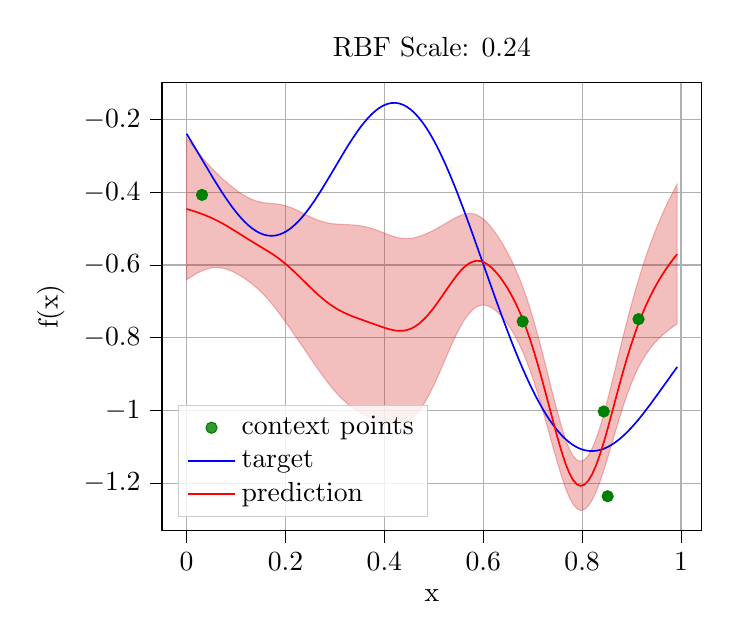
\begin{tikzpicture}

\definecolor{crimson2143940}{RGB}{214,39,40}
\definecolor{darkgray176}{RGB}{176,176,176}
\definecolor{green}{RGB}{0,128,0}
\definecolor{lightgray204}{RGB}{204,204,204}

\begin{axis}[
legend cell align={left},
legend style={
  fill opacity=0.8,
  draw opacity=1,
  text opacity=1,
  at={(0.03,0.03)},
  anchor=south west,
  draw=lightgray204
},
tick align=outside,
tick pos=left,
title={RBF Scale: 0.24},
x grid style={darkgray176},
xlabel={x},
xmajorgrids,
xmin=-0.049609375, xmax=1.041796875,
xtick style={color=black},
y grid style={darkgray176},
ylabel={f(x)},
ymajorgrids,
ymin=-1.33123987838626, ymax=-0.0979588784277439,
ytick style={color=black}
]
\addplot [draw=green, fill=green, mark=*, only marks]
table{%
x  y
0.03125 -0.407177895307541
0.6796875 -0.755326390266418
0.84375 -1.00302398204803
0.8515625 -1.23615598678589
0.9140625 -0.74896651506424
};
\addlegendentry{context points}
\path [draw=crimson2143940, fill=crimson2143940, opacity=0.3]
(axis cs:0,-0.250930607318878)
--(axis cs:0,-0.640730917453766)
--(axis cs:0.0078125,-0.633859992027283)
--(axis cs:0.015625,-0.627196192741394)
--(axis cs:0.0234375,-0.62118262052536)
--(axis cs:0.03125,-0.616000950336456)
--(axis cs:0.0390625,-0.611818730831146)
--(axis cs:0.046875,-0.608944535255432)
--(axis cs:0.0546875,-0.607336521148682)
--(axis cs:0.0625,-0.607151627540588)
--(axis cs:0.0703125,-0.608184814453125)
--(axis cs:0.078125,-0.610496759414673)
--(axis cs:0.0859375,-0.613978207111359)
--(axis cs:0.09375,-0.618479430675507)
--(axis cs:0.1015625,-0.623830258846283)
--(axis cs:0.109375,-0.63003146648407)
--(axis cs:0.1171875,-0.636853158473969)
--(axis cs:0.125,-0.644419312477112)
--(axis cs:0.1328125,-0.652554869651794)
--(axis cs:0.140625,-0.661490797996521)
--(axis cs:0.1484375,-0.671187043190002)
--(axis cs:0.15625,-0.681749701499939)
--(axis cs:0.1640625,-0.693382322788239)
--(axis cs:0.171875,-0.705816626548767)
--(axis cs:0.1796875,-0.719140946865082)
--(axis cs:0.1875,-0.733110666275024)
--(axis cs:0.1953125,-0.747758686542511)
--(axis cs:0.203125,-0.762580931186676)
--(axis cs:0.2109375,-0.777686238288879)
--(axis cs:0.21875,-0.793001651763916)
--(axis cs:0.2265625,-0.808491468429565)
--(axis cs:0.234375,-0.824082791805267)
--(axis cs:0.2421875,-0.83976536989212)
--(axis cs:0.25,-0.855321228504181)
--(axis cs:0.2578125,-0.870914161205292)
--(axis cs:0.265625,-0.886180996894836)
--(axis cs:0.2734375,-0.901079416275024)
--(axis cs:0.28125,-0.915595293045044)
--(axis cs:0.2890625,-0.929402768611908)
--(axis cs:0.296875,-0.942435264587402)
--(axis cs:0.3046875,-0.95461243391037)
--(axis cs:0.3125,-0.965697228908539)
--(axis cs:0.3203125,-0.97586864233017)
--(axis cs:0.328125,-0.984927296638489)
--(axis cs:0.3359375,-0.992944240570068)
--(axis cs:0.34375,-1.00014662742615)
--(axis cs:0.3515625,-1.0063636302948)
--(axis cs:0.359375,-1.01205146312714)
--(axis cs:0.3671875,-1.01695346832275)
--(axis cs:0.375,-1.02153432369232)
--(axis cs:0.3828125,-1.02554488182068)
--(axis cs:0.390625,-1.02914011478424)
--(axis cs:0.3984375,-1.03231000900269)
--(axis cs:0.40625,-1.03489661216736)
--(axis cs:0.4140625,-1.03669393062592)
--(axis cs:0.421875,-1.03751289844513)
--(axis cs:0.4296875,-1.03697884082794)
--(axis cs:0.4375,-1.03487956523895)
--(axis cs:0.4453125,-1.0307332277298)
--(axis cs:0.453125,-1.02428388595581)
--(axis cs:0.4609375,-1.01535272598267)
--(axis cs:0.46875,-1.00370287895203)
--(axis cs:0.4765625,-0.989284038543701)
--(axis cs:0.484375,-0.97213751077652)
--(axis cs:0.4921875,-0.952554225921631)
--(axis cs:0.5,-0.930996060371399)
--(axis cs:0.5078125,-0.907617330551147)
--(axis cs:0.515625,-0.883336961269379)
--(axis cs:0.5234375,-0.858528554439545)
--(axis cs:0.53125,-0.833992958068848)
--(axis cs:0.5390625,-0.810136437416077)
--(axis cs:0.546875,-0.787797391414642)
--(axis cs:0.5546875,-0.767414689064026)
--(axis cs:0.5625,-0.749588787555695)
--(axis cs:0.5703125,-0.734901070594788)
--(axis cs:0.578125,-0.723420202732086)
--(axis cs:0.5859375,-0.715482294559479)
--(axis cs:0.59375,-0.711083948612213)
--(axis cs:0.6015625,-0.710155129432678)
--(axis cs:0.609375,-0.712443351745605)
--(axis cs:0.6171875,-0.717623710632324)
--(axis cs:0.625,-0.725254058837891)
--(axis cs:0.6328125,-0.735010027885437)
--(axis cs:0.640625,-0.746909916400909)
--(axis cs:0.6484375,-0.76075953245163)
--(axis cs:0.65625,-0.776628911495209)
--(axis cs:0.6640625,-0.794695615768433)
--(axis cs:0.671875,-0.815196454524994)
--(axis cs:0.6796875,-0.838164627552032)
--(axis cs:0.6875,-0.863923490047455)
--(axis cs:0.6953125,-0.892471551895142)
--(axis cs:0.703125,-0.923714697360992)
--(axis cs:0.7109375,-0.957194983959198)
--(axis cs:0.71875,-0.992721259593964)
--(axis cs:0.7265625,-1.02975845336914)
--(axis cs:0.734375,-1.06799495220184)
--(axis cs:0.7421875,-1.10629320144653)
--(axis cs:0.75,-1.1437326669693)
--(axis cs:0.7578125,-1.17895996570587)
--(axis cs:0.765625,-1.21084880828857)
--(axis cs:0.7734375,-1.23742973804474)
--(axis cs:0.78125,-1.2574565410614)
--(axis cs:0.7890625,-1.27017939090729)
--(axis cs:0.796875,-1.27518165111542)
--(axis cs:0.8046875,-1.27259004116058)
--(axis cs:0.8125,-1.26275634765625)
--(axis cs:0.8203125,-1.24641215801239)
--(axis cs:0.828125,-1.22415959835052)
--(axis cs:0.8359375,-1.19658672809601)
--(axis cs:0.84375,-1.16521573066711)
--(axis cs:0.8515625,-1.13081729412079)
--(axis cs:0.859375,-1.09487748146057)
--(axis cs:0.8671875,-1.05874645709991)
--(axis cs:0.875,-1.02319896221161)
--(axis cs:0.8828125,-0.989393770694733)
--(axis cs:0.890625,-0.958279430866241)
--(axis cs:0.8984375,-0.929746627807617)
--(axis cs:0.90625,-0.904251635074615)
--(axis cs:0.9140625,-0.881588757038116)
--(axis cs:0.921875,-0.861983895301819)
--(axis cs:0.9296875,-0.844778716564178)
--(axis cs:0.9375,-0.829801440238953)
--(axis cs:0.9453125,-0.816671371459961)
--(axis cs:0.953125,-0.805207371711731)
--(axis cs:0.9609375,-0.794865131378174)
--(axis cs:0.96875,-0.785673022270203)
--(axis cs:0.9765625,-0.777227640151978)
--(axis cs:0.984375,-0.769353568553925)
--(axis cs:0.9921875,-0.762062191963196)
--(axis cs:0.9921875,-0.378130197525024)
--(axis cs:0.9921875,-0.378130197525024)
--(axis cs:0.984375,-0.397635996341705)
--(axis cs:0.9765625,-0.418408632278442)
--(axis cs:0.96875,-0.440363764762878)
--(axis cs:0.9609375,-0.463838934898376)
--(axis cs:0.953125,-0.488938212394714)
--(axis cs:0.9453125,-0.515513181686401)
--(axis cs:0.9375,-0.543933033943176)
--(axis cs:0.9296875,-0.574054539203644)
--(axis cs:0.921875,-0.606221556663513)
--(axis cs:0.9140625,-0.640274941921234)
--(axis cs:0.90625,-0.676502525806427)
--(axis cs:0.8984375,-0.714702486991882)
--(axis cs:0.890625,-0.755001962184906)
--(axis cs:0.8828125,-0.796770036220551)
--(axis cs:0.875,-0.840136528015137)
--(axis cs:0.8671875,-0.884225785732269)
--(axis cs:0.859375,-0.927876234054565)
--(axis cs:0.8515625,-0.970404505729675)
--(axis cs:0.84375,-1.01057267189026)
--(axis cs:0.8359375,-1.04689133167267)
--(axis cs:0.828125,-1.0786749124527)
--(axis cs:0.8203125,-1.10449826717377)
--(axis cs:0.8125,-1.1237518787384)
--(axis cs:0.8046875,-1.13589465618134)
--(axis cs:0.796875,-1.14020526409149)
--(axis cs:0.7890625,-1.13629734516144)
--(axis cs:0.78125,-1.1240086555481)
--(axis cs:0.7734375,-1.10368025302887)
--(axis cs:0.765625,-1.07604169845581)
--(axis cs:0.7578125,-1.0422819852829)
--(axis cs:0.75,-1.00433814525604)
--(axis cs:0.7421875,-0.963415682315826)
--(axis cs:0.734375,-0.920958340167999)
--(axis cs:0.7265625,-0.878139317035675)
--(axis cs:0.71875,-0.836279690265656)
--(axis cs:0.7109375,-0.795972168445587)
--(axis cs:0.703125,-0.757865130901337)
--(axis cs:0.6953125,-0.722171783447266)
--(axis cs:0.6875,-0.689338147640228)
--(axis cs:0.6796875,-0.659409463405609)
--(axis cs:0.671875,-0.632254421710968)
--(axis cs:0.6640625,-0.607474803924561)
--(axis cs:0.65625,-0.584899365901947)
--(axis cs:0.6484375,-0.564298808574677)
--(axis cs:0.640625,-0.545359909534454)
--(axis cs:0.6328125,-0.527886390686035)
--(axis cs:0.625,-0.512099146842957)
--(axis cs:0.6171875,-0.49781060218811)
--(axis cs:0.609375,-0.485319972038269)
--(axis cs:0.6015625,-0.475011557340622)
--(axis cs:0.59375,-0.467062890529633)
--(axis cs:0.5859375,-0.461590826511383)
--(axis cs:0.578125,-0.458748161792755)
--(axis cs:0.5703125,-0.458251565694809)
--(axis cs:0.5625,-0.459850490093231)
--(axis cs:0.5546875,-0.463246494531631)
--(axis cs:0.546875,-0.468038260936737)
--(axis cs:0.5390625,-0.473695188760757)
--(axis cs:0.53125,-0.479872584342957)
--(axis cs:0.5234375,-0.486108243465424)
--(axis cs:0.515625,-0.492361485958099)
--(axis cs:0.5078125,-0.498368978500366)
--(axis cs:0.5,-0.504043102264404)
--(axis cs:0.4921875,-0.509313941001892)
--(axis cs:0.484375,-0.514232099056244)
--(axis cs:0.4765625,-0.518527388572693)
--(axis cs:0.46875,-0.522159576416016)
--(axis cs:0.4609375,-0.524899423122406)
--(axis cs:0.453125,-0.526684880256653)
--(axis cs:0.4453125,-0.527431130409241)
--(axis cs:0.4375,-0.526866674423218)
--(axis cs:0.4296875,-0.525280833244324)
--(axis cs:0.421875,-0.522766709327698)
--(axis cs:0.4140625,-0.51939594745636)
--(axis cs:0.40625,-0.515507698059082)
--(axis cs:0.3984375,-0.511346638202667)
--(axis cs:0.390625,-0.507187604904175)
--(axis cs:0.3828125,-0.503254771232605)
--(axis cs:0.375,-0.499776214361191)
--(axis cs:0.3671875,-0.496675848960876)
--(axis cs:0.359375,-0.494167000055313)
--(axis cs:0.3515625,-0.49219936132431)
--(axis cs:0.34375,-0.490722835063934)
--(axis cs:0.3359375,-0.489744275808334)
--(axis cs:0.328125,-0.489222019910812)
--(axis cs:0.3203125,-0.488706648349762)
--(axis cs:0.3125,-0.488244235515594)
--(axis cs:0.3046875,-0.48769873380661)
--(axis cs:0.296875,-0.486690640449524)
--(axis cs:0.2890625,-0.48519104719162)
--(axis cs:0.28125,-0.483079791069031)
--(axis cs:0.2734375,-0.480152010917664)
--(axis cs:0.265625,-0.47656786441803)
--(axis cs:0.2578125,-0.472314178943634)
--(axis cs:0.25,-0.46744304895401)
--(axis cs:0.2421875,-0.462269604206085)
--(axis cs:0.234375,-0.456869542598724)
--(axis cs:0.2265625,-0.451517224311829)
--(axis cs:0.21875,-0.446468681097031)
--(axis cs:0.2109375,-0.441970109939575)
--(axis cs:0.203125,-0.438278138637543)
--(axis cs:0.1953125,-0.435328543186188)
--(axis cs:0.1875,-0.433210968971252)
--(axis cs:0.1796875,-0.431842029094696)
--(axis cs:0.171875,-0.430903166532516)
--(axis cs:0.1640625,-0.429937541484833)
--(axis cs:0.15625,-0.428580969572067)
--(axis cs:0.1484375,-0.42659604549408)
--(axis cs:0.140625,-0.42373725771904)
--(axis cs:0.1328125,-0.419825077056885)
--(axis cs:0.125,-0.414967656135559)
--(axis cs:0.1171875,-0.409091651439667)
--(axis cs:0.109375,-0.402506738901138)
--(axis cs:0.1015625,-0.395080178976059)
--(axis cs:0.09375,-0.387064039707184)
--(axis cs:0.0859375,-0.378439962863922)
--(axis cs:0.078125,-0.369322419166565)
--(axis cs:0.0703125,-0.359727382659912)
--(axis cs:0.0625,-0.349644422531128)
--(axis cs:0.0546875,-0.338979005813599)
--(axis cs:0.046875,-0.327670931816101)
--(axis cs:0.0390625,-0.315846145153046)
--(axis cs:0.03125,-0.303451001644135)
--(axis cs:0.0234375,-0.290524899959564)
--(axis cs:0.015625,-0.27738082408905)
--(axis cs:0.0078125,-0.264075964689255)
--(axis cs:0,-0.250930607318878)
--cycle;

\addplot [semithick, blue]
table {%
0 -0.238928914070129
0.015625 -0.274168968200684
0.0546875 -0.363261818885803
0.0703125 -0.397175073623657
0.078125 -0.413298010826111
0.0859375 -0.428702235221863
0.09375 -0.443266153335571
0.1015625 -0.456871271133423
0.109375 -0.469402194023132
0.1171875 -0.48075008392334
0.125 -0.490813255310059
0.1328125 -0.499498605728149
0.140625 -0.506723403930664
0.1484375 -0.512415885925293
0.15625 -0.516517162322998
0.1640625 -0.518981575965881
0.171875 -0.519777894020081
0.1796875 -0.518889904022217
0.1875 -0.516316294670105
0.1953125 -0.512071967124939
0.203125 -0.506187677383423
0.2109375 -0.498709440231323
0.21875 -0.489699602127075
0.2265625 -0.479235410690308
0.234375 -0.467408061027527
0.2421875 -0.454323530197144
0.25 -0.440100193023682
0.2578125 -0.424868226051331
0.265625 -0.408768892288208
0.2734375 -0.391952157020569
0.2890625 -0.356808423995972
0.3203125 -0.285237073898315
0.328125 -0.268092751502991
0.3359375 -0.251592636108398
0.34375 -0.235902667045593
0.3515625 -0.221182823181152
0.359375 -0.207585096359253
0.3671875 -0.195252656936646
0.375 -0.184318780899048
0.3828125 -0.17490541934967
0.390625 -0.167122483253479
0.3984375 -0.161066055297852
0.40625 -0.156819701194763
0.4140625 -0.154451966285706
0.421875 -0.154017090797424
0.4296875 -0.155554294586182
0.4375 -0.159087777137756
0.4453125 -0.164627552032471
0.453125 -0.172167778015137
0.4609375 -0.181689739227295
0.46875 -0.193159818649292
0.4765625 -0.206531763076782
0.484375 -0.221746683120728
0.4921875 -0.238733530044556
0.5 -0.257411122322083
0.5078125 -0.277687907218933
0.515625 -0.299463510513306
0.5234375 -0.322629809379578
0.53125 -0.347071409225464
0.5390625 -0.372668266296387
0.546875 -0.39929461479187
0.5625 -0.455116510391235
0.578125 -0.513481259346008
0.6015625 -0.603466510772705
0.625 -0.693280100822449
0.640625 -0.751449465751648
0.65625 -0.807232141494751
0.6640625 -0.83398175239563
0.671875 -0.859850883483887
0.6796875 -0.884757280349731
0.6875 -0.908624887466431
0.6953125 -0.931384563446045
0.703125 -0.952972412109375
0.7109375 -0.973332047462463
0.71875 -0.992412328720093
0.7265625 -1.01016902923584
0.734375 -1.02656364440918
0.7421875 -1.0415632724762
0.75 -1.05514228343964
0.7578125 -1.06727957725525
0.765625 -1.07796061038971
0.7734375 -1.08717620372772
0.78125 -1.09492325782776
0.7890625 -1.10120356082916
0.796875 -1.10602521896362
0.8046875 -1.10940110683441
0.8125 -1.11134994029999
0.8203125 -1.11189615726471
0.828125 -1.11106884479523
0.8359375 -1.10890305042267
0.84375 -1.10543823242188
0.8515625 -1.1007205247879
0.859375 -1.09479975700378
0.8671875 -1.0877320766449
0.875 -1.07957780361176
0.8828125 -1.07040226459503
0.890625 -1.06027555465698
0.8984375 -1.04927217960358
0.90625 -1.03747117519379
0.9140625 -1.0249547958374
0.921875 -1.01180934906006
0.9375 -0.983991622924805
0.953125 -0.954761743545532
0.9921875 -0.880557060241699
};
\addlegendentry{target}
\addplot [semithick, red]
table {%
0 -0.445830821990967
0.015625 -0.452288508415222
0.0234375 -0.455853700637817
0.0390625 -0.463832378387451
0.046875 -0.468307733535767
0.0546875 -0.47315776348114
0.0625 -0.478398084640503
0.0703125 -0.483956098556519
0.078125 -0.489909648895264
0.09375 -0.502771735191345
0.140625 -0.542613983154297
0.1640625 -0.561659932136536
0.171875 -0.568359851837158
0.1796875 -0.575491428375244
0.1875 -0.583160877227783
0.1953125 -0.591543674468994
0.203125 -0.600429534912109
0.2109375 -0.609828233718872
0.2265625 -0.630004405975342
0.2578125 -0.671614170074463
0.265625 -0.681374430656433
0.2734375 -0.690615653991699
0.28125 -0.699337482452393
0.2890625 -0.707296848297119
0.296875 -0.714562892913818
0.3046875 -0.721155643463135
0.3125 -0.726970672607422
0.3203125 -0.732287645339966
0.328125 -0.737074613571167
0.34375 -0.745434761047363
0.375 -0.760655283927917
0.3984375 -0.771828293800354
0.40625 -0.77520215511322
0.4140625 -0.778044939041138
0.421875 -0.780139803886414
0.4296875 -0.781129837036133
0.4375 -0.78087306022644
0.4453125 -0.779082179069519
0.453125 -0.775484323501587
0.4609375 -0.770126104354858
0.46875 -0.762931227684021
0.4765625 -0.753905773162842
0.484375 -0.743184804916382
0.4921875 -0.730934143066406
0.5 -0.717519521713257
0.5078125 -0.702993154525757
0.5234375 -0.672318458557129
0.5390625 -0.641915798187256
0.546875 -0.627917766571045
0.5546875 -0.615330576896667
0.5625 -0.604719638824463
0.5703125 -0.596576333045959
0.578125 -0.591084241867065
0.5859375 -0.588536500930786
0.59375 -0.589073419570923
0.6015625 -0.592583417892456
0.609375 -0.598881721496582
0.6171875 -0.607717156410217
0.625 -0.618676662445068
0.6328125 -0.631448268890381
0.640625 -0.646134853363037
0.6484375 -0.662529230117798
0.65625 -0.680764198303223
0.6640625 -0.701085209846497
0.671875 -0.723725438117981
0.6796875 -0.748787045478821
0.6875 -0.776630878448486
0.6953125 -0.807321667671204
0.703125 -0.840789914131165
0.7109375 -0.876583576202393
0.71875 -0.91450047492981
0.734375 -0.994476675987244
0.75 -1.07403540611267
0.7578125 -1.11062097549438
0.765625 -1.14344525337219
0.7734375 -1.1705549955368
0.78125 -1.19073259830475
0.7890625 -1.20323836803436
0.796875 -1.20769345760345
0.8046875 -1.20424234867096
0.8125 -1.19325411319733
0.8203125 -1.17545521259308
0.828125 -1.15141725540161
0.8359375 -1.12173902988434
0.84375 -1.08789420127869
0.8515625 -1.05061089992523
0.8671875 -0.97148609161377
0.875 -0.931667804718018
0.8828125 -0.893081903457642
0.890625 -0.856640696525574
0.8984375 -0.822224617004395
0.90625 -0.790377140045166
0.9140625 -0.760931849479675
0.921875 -0.734102725982666
0.9296875 -0.709416627883911
0.9375 -0.686867237091064
0.9453125 -0.666092276573181
0.953125 -0.647072792053223
0.9609375 -0.62935209274292
0.96875 -0.613018393516541
0.9765625 -0.59781813621521
0.984375 -0.583494782447815
0.9921875 -0.570096254348755
};
\addlegendentry{prediction}
\end{axis}

\end{tikzpicture}

		% This file was created with matplot2tikz v0.4.0.
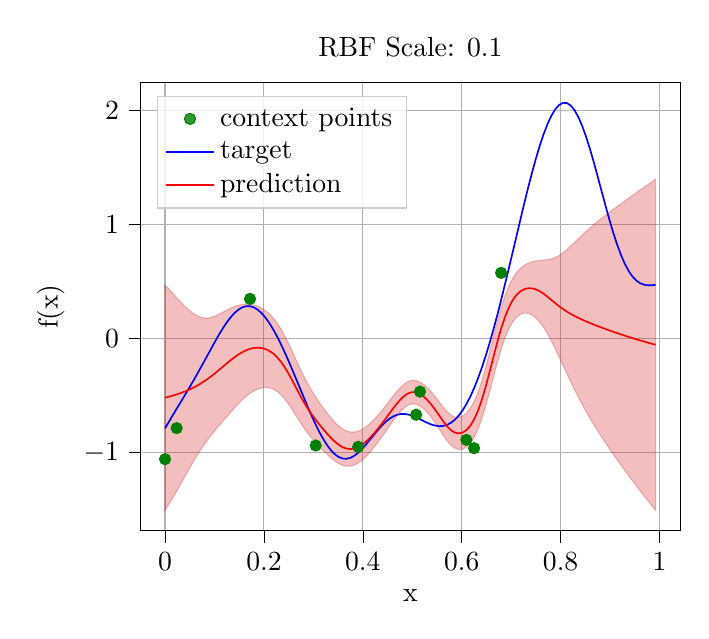
\begin{tikzpicture}

\definecolor{crimson2143940}{RGB}{214,39,40}
\definecolor{darkgray176}{RGB}{176,176,176}
\definecolor{green}{RGB}{0,128,0}
\definecolor{lightgray204}{RGB}{204,204,204}

\begin{axis}[
legend cell align={left},
legend style={
  fill opacity=0.8,
  draw opacity=1,
  text opacity=1,
  at={(0.03,0.97)},
  anchor=north west,
  draw=lightgray204
},
tick align=outside,
tick pos=left,
title={RBF Scale: 0.1},
x grid style={darkgray176},
xlabel={x},
xmajorgrids,
xmin=-0.049609375, xmax=1.041796875,
xtick style={color=black},
y grid style={darkgray176},
ylabel={f(x)},
ymajorgrids,
ymin=-1.68710995316505, ymax=2.24367321133614,
ytick style={color=black}
]
\addplot [draw=green, fill=green, mark=*, only marks]
table{%
x  y
0 -1.05894541740417
0.0234375 -0.786890625953674
0.171875 0.346168965101242
0.3046875 -0.939141511917114
0.390625 -0.950726628303528
0.5078125 -0.669203221797943
0.515625 -0.466711491346359
0.609375 -0.889861762523651
0.625 -0.962745904922485
0.6796875 0.574347078800201
};
\addlegendentry{context points}
\path [draw=crimson2143940, fill=crimson2143940, opacity=0.3]
(axis cs:0,0.466936469078064)
--(axis cs:0,-1.5077155828476)
--(axis cs:0.0078125,-1.45429039001465)
--(axis cs:0.015625,-1.39851355552673)
--(axis cs:0.0234375,-1.34039950370789)
--(axis cs:0.03125,-1.28074407577515)
--(axis cs:0.0390625,-1.21997404098511)
--(axis cs:0.046875,-1.15968155860901)
--(axis cs:0.0546875,-1.1000953912735)
--(axis cs:0.0625,-1.04266059398651)
--(axis cs:0.0703125,-0.988298416137695)
--(axis cs:0.078125,-0.937345683574677)
--(axis cs:0.0859375,-0.890078723430634)
--(axis cs:0.09375,-0.846068561077118)
--(axis cs:0.1015625,-0.804442346096039)
--(axis cs:0.109375,-0.764432489871979)
--(axis cs:0.1171875,-0.725270390510559)
--(axis cs:0.125,-0.685942411422729)
--(axis cs:0.1328125,-0.647220373153687)
--(axis cs:0.140625,-0.609138965606689)
--(axis cs:0.1484375,-0.572738409042358)
--(axis cs:0.15625,-0.538766622543335)
--(axis cs:0.1640625,-0.508454084396362)
--(axis cs:0.171875,-0.482283800840378)
--(axis cs:0.1796875,-0.461010307073593)
--(axis cs:0.1875,-0.444985568523407)
--(axis cs:0.1953125,-0.434858381748199)
--(axis cs:0.203125,-0.43099445104599)
--(axis cs:0.2109375,-0.43435400724411)
--(axis cs:0.21875,-0.445072084665298)
--(axis cs:0.2265625,-0.464781999588013)
--(axis cs:0.234375,-0.493345886468887)
--(axis cs:0.2421875,-0.531016945838928)
--(axis cs:0.25,-0.576609671115875)
--(axis cs:0.2578125,-0.628556728363037)
--(axis cs:0.265625,-0.682785987854004)
--(axis cs:0.2734375,-0.736451089382172)
--(axis cs:0.28125,-0.787149310112)
--(axis cs:0.2890625,-0.833009481430054)
--(axis cs:0.296875,-0.875112473964691)
--(axis cs:0.3046875,-0.913407564163208)
--(axis cs:0.3125,-0.950050175189972)
--(axis cs:0.3203125,-0.984746277332306)
--(axis cs:0.328125,-1.0178142786026)
--(axis cs:0.3359375,-1.04877972602844)
--(axis cs:0.34375,-1.07629132270813)
--(axis cs:0.3515625,-1.09823286533356)
--(axis cs:0.359375,-1.11379098892212)
--(axis cs:0.3671875,-1.12094163894653)
--(axis cs:0.375,-1.11989510059357)
--(axis cs:0.3828125,-1.11036384105682)
--(axis cs:0.390625,-1.09249365329742)
--(axis cs:0.3984375,-1.06777000427246)
--(axis cs:0.40625,-1.03643774986267)
--(axis cs:0.4140625,-0.999989628791809)
--(axis cs:0.421875,-0.95942759513855)
--(axis cs:0.4296875,-0.915365040302277)
--(axis cs:0.4375,-0.868820130825043)
--(axis cs:0.4453125,-0.820839464664459)
--(axis cs:0.453125,-0.771953880786896)
--(axis cs:0.4609375,-0.723901212215424)
--(axis cs:0.46875,-0.678668200969696)
--(axis cs:0.4765625,-0.638667821884155)
--(axis cs:0.484375,-0.606283605098724)
--(axis cs:0.4921875,-0.584081709384918)
--(axis cs:0.5,-0.574225246906281)
--(axis cs:0.5078125,-0.577383100986481)
--(axis cs:0.515625,-0.593112289905548)
--(axis cs:0.5234375,-0.618839800357819)
--(axis cs:0.53125,-0.653621912002563)
--(axis cs:0.5390625,-0.695764601230621)
--(axis cs:0.546875,-0.744167804718018)
--(axis cs:0.5546875,-0.796925187110901)
--(axis cs:0.5625,-0.849908709526062)
--(axis cs:0.5703125,-0.898299336433411)
--(axis cs:0.578125,-0.936954617500305)
--(axis cs:0.5859375,-0.962685942649841)
--(axis cs:0.59375,-0.974236965179443)
--(axis cs:0.6015625,-0.971407473087311)
--(axis cs:0.609375,-0.95343679189682)
--(axis cs:0.6171875,-0.919699370861053)
--(axis cs:0.625,-0.86798620223999)
--(axis cs:0.6328125,-0.796385049819946)
--(axis cs:0.640625,-0.703916490077972)
--(axis cs:0.6484375,-0.593245983123779)
--(axis cs:0.65625,-0.468912541866302)
--(axis cs:0.6640625,-0.339601397514343)
--(axis cs:0.671875,-0.212962821125984)
--(axis cs:0.6796875,-0.0971233695745468)
--(axis cs:0.6875,0.00304484367370605)
--(axis cs:0.6953125,0.0838107913732529)
--(axis cs:0.703125,0.144310757517815)
--(axis cs:0.7109375,0.186380952596664)
--(axis cs:0.71875,0.211371257901192)
--(axis cs:0.7265625,0.221955507993698)
--(axis cs:0.734375,0.219658568501472)
--(axis cs:0.7421875,0.205250307917595)
--(axis cs:0.75,0.179815053939819)
--(axis cs:0.7578125,0.143320083618164)
--(axis cs:0.765625,0.0965725779533386)
--(axis cs:0.7734375,0.0405098795890808)
--(axis cs:0.78125,-0.022766500711441)
--(axis cs:0.7890625,-0.0911297202110291)
--(axis cs:0.796875,-0.163232684135437)
--(axis cs:0.8046875,-0.235990703105927)
--(axis cs:0.8125,-0.308793604373932)
--(axis cs:0.8203125,-0.380035996437073)
--(axis cs:0.828125,-0.448977053165436)
--(axis cs:0.8359375,-0.515420019626617)
--(axis cs:0.84375,-0.579192161560059)
--(axis cs:0.8515625,-0.640487432479858)
--(axis cs:0.859375,-0.699179232120514)
--(axis cs:0.8671875,-0.755874395370483)
--(axis cs:0.875,-0.810374796390533)
--(axis cs:0.8828125,-0.863472044467926)
--(axis cs:0.890625,-0.914956390857697)
--(axis cs:0.8984375,-0.965498089790344)
--(axis cs:0.90625,-1.0147157907486)
--(axis cs:0.9140625,-1.06297731399536)
--(axis cs:0.921875,-1.11029350757599)
--(axis cs:0.9296875,-1.15693938732147)
--(axis cs:0.9375,-1.20290887355804)
--(axis cs:0.9453125,-1.2482727766037)
--(axis cs:0.953125,-1.29299557209015)
--(axis cs:0.9609375,-1.33724105358124)
--(axis cs:0.96875,-1.38080072402954)
--(axis cs:0.9765625,-1.42374575138092)
--(axis cs:0.984375,-1.46619164943695)
--(axis cs:0.9921875,-1.50843799114227)
--(axis cs:0.9921875,1.39648067951202)
--(axis cs:0.9921875,1.39648067951202)
--(axis cs:0.984375,1.37270128726959)
--(axis cs:0.9765625,1.34870302677155)
--(axis cs:0.96875,1.32499694824219)
--(axis cs:0.9609375,1.3012775182724)
--(axis cs:0.953125,1.27720630168915)
--(axis cs:0.9453125,1.25336635112762)
--(axis cs:0.9375,1.22920787334442)
--(axis cs:0.9296875,1.20477879047394)
--(axis cs:0.921875,1.18044149875641)
--(axis cs:0.9140625,1.1559054851532)
--(axis cs:0.90625,1.13085114955902)
--(axis cs:0.8984375,1.10533702373505)
--(axis cs:0.890625,1.07939910888672)
--(axis cs:0.8828125,1.05293726921082)
--(axis cs:0.875,1.02552580833435)
--(axis cs:0.8671875,0.997525691986084)
--(axis cs:0.859375,0.968298494815826)
--(axis cs:0.8515625,0.938216686248779)
--(axis cs:0.84375,0.906777143478394)
--(axis cs:0.8359375,0.874912321567535)
--(axis cs:0.828125,0.842131197452545)
--(axis cs:0.8203125,0.81005585193634)
--(axis cs:0.8125,0.779105007648468)
--(axis cs:0.8046875,0.750905454158783)
--(axis cs:0.796875,0.727161526679993)
--(axis cs:0.7890625,0.70903605222702)
--(axis cs:0.78125,0.696734309196472)
--(axis cs:0.7734375,0.689626753330231)
--(axis cs:0.765625,0.686047375202179)
--(axis cs:0.7578125,0.683353662490845)
--(axis cs:0.75,0.679218769073486)
--(axis cs:0.7421875,0.67181533575058)
--(axis cs:0.734375,0.659730494022369)
--(axis cs:0.7265625,0.641308307647705)
--(axis cs:0.71875,0.614768445491791)
--(axis cs:0.7109375,0.577841639518738)
--(axis cs:0.703125,0.52713531255722)
--(axis cs:0.6953125,0.460148811340332)
--(axis cs:0.6875,0.37404990196228)
--(axis cs:0.6796875,0.268450498580933)
--(axis cs:0.671875,0.146601155400276)
--(axis cs:0.6640625,0.0131790637969971)
--(axis cs:0.65625,-0.123594477772713)
--(axis cs:0.6484375,-0.255783289670944)
--(axis cs:0.640625,-0.374287664890289)
--(axis cs:0.6328125,-0.474637508392334)
--(axis cs:0.625,-0.554044008255005)
--(axis cs:0.6171875,-0.613575279712677)
--(axis cs:0.609375,-0.655154049396515)
--(axis cs:0.6015625,-0.681211173534393)
--(axis cs:0.59375,-0.692360162734985)
--(axis cs:0.5859375,-0.68938934803009)
--(axis cs:0.578125,-0.672417521476746)
--(axis cs:0.5703125,-0.642618536949158)
--(axis cs:0.5625,-0.602903008460999)
--(axis cs:0.5546875,-0.558262944221497)
--(axis cs:0.546875,-0.513214945793152)
--(axis cs:0.5390625,-0.471727550029755)
--(axis cs:0.53125,-0.435463041067123)
--(axis cs:0.5234375,-0.40542083978653)
--(axis cs:0.515625,-0.383187741041183)
--(axis cs:0.5078125,-0.369705975055695)
--(axis cs:0.5,-0.367582619190216)
--(axis cs:0.4921875,-0.377400189638138)
--(axis cs:0.484375,-0.398530781269073)
--(axis cs:0.4765625,-0.428953409194946)
--(axis cs:0.46875,-0.466127455234528)
--(axis cs:0.4609375,-0.507832467556)
--(axis cs:0.453125,-0.551548898220062)
--(axis cs:0.4453125,-0.595349729061127)
--(axis cs:0.4375,-0.637509882450104)
--(axis cs:0.4296875,-0.677495896816254)
--(axis cs:0.421875,-0.714276790618896)
--(axis cs:0.4140625,-0.74694287776947)
--(axis cs:0.40625,-0.774952173233032)
--(axis cs:0.3984375,-0.797391295433044)
--(axis cs:0.390625,-0.812851071357727)
--(axis cs:0.3828125,-0.821119368076324)
--(axis cs:0.375,-0.820952951908112)
--(axis cs:0.3671875,-0.81220668554306)
--(axis cs:0.359375,-0.795085668563843)
--(axis cs:0.3515625,-0.769562602043152)
--(axis cs:0.34375,-0.737409591674805)
--(axis cs:0.3359375,-0.699358224868774)
--(axis cs:0.328125,-0.657275795936584)
--(axis cs:0.3203125,-0.612255752086639)
--(axis cs:0.3125,-0.564669549465179)
--(axis cs:0.3046875,-0.513953924179077)
--(axis cs:0.296875,-0.460283577442169)
--(axis cs:0.2890625,-0.401533484458923)
--(axis cs:0.28125,-0.337914824485779)
--(axis cs:0.2734375,-0.268223106861115)
--(axis cs:0.265625,-0.1946020424366)
--(axis cs:0.2578125,-0.119409412145615)
--(axis cs:0.25,-0.0457594990730286)
--(axis cs:0.2421875,0.0223082602024078)
--(axis cs:0.234375,0.0831661522388458)
--(axis cs:0.2265625,0.135301232337952)
--(axis cs:0.21875,0.179327756166458)
--(axis cs:0.2109375,0.214894235134125)
--(axis cs:0.203125,0.243672072887421)
--(axis cs:0.1953125,0.265632927417755)
--(axis cs:0.1875,0.281938016414642)
--(axis cs:0.1796875,0.292997926473618)
--(axis cs:0.171875,0.298938244581223)
--(axis cs:0.1640625,0.300329953432083)
--(axis cs:0.15625,0.297372728586197)
--(axis cs:0.1484375,0.29031503200531)
--(axis cs:0.140625,0.279639691114426)
--(axis cs:0.1328125,0.265678763389587)
--(axis cs:0.125,0.249249070882797)
--(axis cs:0.1171875,0.230940908193588)
--(axis cs:0.109375,0.212967097759247)
--(axis cs:0.1015625,0.196826159954071)
--(axis cs:0.09375,0.184865891933441)
--(axis cs:0.0859375,0.178531467914581)
--(axis cs:0.078125,0.179237306118011)
--(axis cs:0.0703125,0.187754034996033)
--(axis cs:0.0625,0.203322410583496)
--(axis cs:0.0546875,0.226034045219421)
--(axis cs:0.046875,0.253935694694519)
--(axis cs:0.0390625,0.286325991153717)
--(axis cs:0.03125,0.321286678314209)
--(axis cs:0.0234375,0.357901155948639)
--(axis cs:0.015625,0.394938409328461)
--(axis cs:0.0078125,0.431559860706329)
--(axis cs:0,0.466936469078064)
--cycle;

\addplot [semithick, blue]
table {%
0 -0.788702726364136
0.015625 -0.673458337783813
0.046875 -0.448688268661499
0.0625 -0.331692695617676
0.078125 -0.209595203399658
0.1015625 -0.024061918258667
0.109375 0.0348881483078003
0.1171875 0.0904006958007812
0.125 0.141155004501343
0.1328125 0.185845851898193
0.140625 0.223255753517151
0.1484375 0.252320647239685
0.15625 0.272181749343872
0.1640625 0.282225131988525
0.171875 0.282098770141602
0.1796875 0.271716475486755
0.1875 0.25124192237854
0.1953125 0.221060872077942
0.203125 0.181744575500488
0.2109375 0.134008407592773
0.21875 0.0786707401275635
0.2265625 0.0166175365447998
0.234375 -0.0512244701385498
0.2421875 -0.123905181884766
0.25 -0.200456857681274
0.265625 -0.361185669898987
0.2890625 -0.605267643928528
0.296875 -0.682722330093384
0.3046875 -0.756090641021729
0.3125 -0.82404351234436
0.3203125 -0.885273218154907
0.328125 -0.938543915748596
0.3359375 -0.982757806777954
0.34375 -1.01701760292053
0.3515625 -1.04069375991821
0.359375 -1.05347859859467
0.3671875 -1.05543088912964
0.375 -1.04699885845184
0.3828125 -1.0290242433548
0.390625 -1.00271856784821
0.3984375 -0.969618439674377
0.40625 -0.931516170501709
0.4296875 -0.807043194770813
0.4375 -0.768696546554565
0.4453125 -0.734784960746765
0.453125 -0.706592798233032
0.4609375 -0.685020089149475
0.46875 -0.670546770095825
0.4765625 -0.663221120834351
0.484375 -0.66267728805542
0.4921875 -0.668172359466553
0.5 -0.678644776344299
0.5078125 -0.69278621673584
0.515625 -0.709118366241455
0.5234375 -0.726072311401367
0.53125 -0.742062449455261
0.5390625 -0.755549669265747
0.546875 -0.765093564987183
0.5546875 -0.769389033317566
0.5625 -0.767290115356445
0.5703125 -0.757820010185242
0.578125 -0.740172624588013
0.5859375 -0.713705539703369
0.59375 -0.677931308746338
0.6015625 -0.632504820823669
0.609375 -0.577215433120728
0.6171875 -0.511979341506958
0.625 -0.436836838722229
0.6328125 -0.35195255279541
0.640625 -0.257617712020874
0.6484375 -0.154255151748657
0.65625 -0.0424230098724365
0.6640625 0.0771812200546265
0.671875 0.203720450401306
0.6796875 0.33621871471405
0.6953125 0.614522933959961
0.7265625 1.18571674823761
0.734375 1.32232451438904
0.7421875 1.45296692848206
0.75 1.57579874992371
0.7578125 1.68894648551941
0.765625 1.79053568840027
0.7734375 1.87872815132141
0.78125 1.95176839828491
0.7890625 2.00804471969604
0.796875 2.04615831375122
0.8046875 2.06500124931335
0.8125 2.06384181976318
0.8203125 2.04240250587463
0.828125 2.00093245506287
0.8359375 1.94026112556458
0.84375 1.86182570457458
0.8515625 1.76766502857208
0.859375 1.66037786006927
0.8671875 1.54304111003876
0.8828125 1.29217457771301
0.890625 1.16597652435303
0.8984375 1.04403984546661
0.90625 0.929586887359619
0.9140625 0.825360059738159
0.921875 0.733490109443665
0.9296875 0.655404210090637
0.9375 0.591780066490173
0.9453125 0.542546033859253
0.953125 0.506927490234375
0.9609375 0.48353099822998
0.96875 0.470461845397949
0.9765625 0.465458273887634
0.984375 0.46603798866272
0.9921875 0.469641804695129
};
\addlegendentry{target}
\addplot [semithick, red]
table {%
0 -0.520389556884766
0.0078125 -0.511365294456482
0.015625 -0.501787543296814
0.0234375 -0.491249203681946
0.03125 -0.479728698730469
0.0390625 -0.466824054718018
0.046875 -0.45287299156189
0.0546875 -0.437030673027039
0.0625 -0.419669151306152
0.0703125 -0.400272130966187
0.078125 -0.379054188728333
0.0859375 -0.355773687362671
0.09375 -0.330601334571838
0.1015625 -0.303808093070984
0.1171875 -0.247164726257324
0.125 -0.21834659576416
0.1328125 -0.190770864486694
0.140625 -0.164749622344971
0.1484375 -0.141211748123169
0.15625 -0.120697021484375
0.1640625 -0.104062080383301
0.171875 -0.0916727781295776
0.1796875 -0.0840061902999878
0.1875 -0.0815237760543823
0.1953125 -0.0846127271652222
0.203125 -0.0936611890792847
0.2109375 -0.109729886054993
0.21875 -0.132872104644775
0.2265625 -0.164740324020386
0.234375 -0.205089807510376
0.2421875 -0.254354357719421
0.25 -0.311184644699097
0.2578125 -0.373983144760132
0.2734375 -0.502337098121643
0.28125 -0.562532067298889
0.2890625 -0.617271423339844
0.296875 -0.66769802570343
0.3046875 -0.713680744171143
0.3125 -0.757359862327576
0.3203125 -0.798501014709473
0.328125 -0.837545037269592
0.3359375 -0.874068975448608
0.34375 -0.906850457191467
0.3515625 -0.933897733688354
0.359375 -0.954438328742981
0.3671875 -0.966574192047119
0.375 -0.970423936843872
0.3828125 -0.965741634368896
0.390625 -0.952672362327576
0.3984375 -0.932580709457397
0.40625 -0.905694961547852
0.4140625 -0.87346625328064
0.421875 -0.836852192878723
0.4296875 -0.796430468559265
0.4375 -0.753165006637573
0.453125 -0.661751389503479
0.4609375 -0.615866899490356
0.46875 -0.572397828102112
0.4765625 -0.533810615539551
0.484375 -0.502407193183899
0.4921875 -0.480741024017334
0.5 -0.470903873443604
0.5078125 -0.473544597625732
0.515625 -0.488150000572205
0.5234375 -0.512130260467529
0.53125 -0.544542551040649
0.5390625 -0.583746075630188
0.546875 -0.628691434860229
0.5625 -0.72640585899353
0.5703125 -0.770458936691284
0.578125 -0.804686069488525
0.5859375 -0.826037645339966
0.59375 -0.833298563957214
0.6015625 -0.826309323310852
0.609375 -0.804295420646667
0.6171875 -0.766637325286865
0.625 -0.711015105247498
0.6328125 -0.63551127910614
0.640625 -0.539102077484131
0.6484375 -0.424514651298523
0.65625 -0.296253442764282
0.671875 -0.033180832862854
0.6796875 0.0856635570526123
0.6875 0.188547372817993
0.6953125 0.271979808807373
0.703125 0.335723042488098
0.7109375 0.382111310958862
0.71875 0.413069844245911
0.7265625 0.431631922721863
0.734375 0.43969452381134
0.7421875 0.438532829284668
0.75 0.429516911506653
0.7578125 0.413336873054504
0.765625 0.391309976577759
0.7734375 0.365068316459656
0.7890625 0.308953166007996
0.796875 0.281964421272278
0.8046875 0.257457375526428
0.8125 0.235155701637268
0.8203125 0.215009927749634
0.828125 0.196577072143555
0.8359375 0.179746150970459
0.84375 0.163792490959167
0.8515625 0.14886462688446
0.859375 0.134559631347656
0.8671875 0.1208256483078
0.8828125 0.0947326421737671
0.8984375 0.0699194669723511
0.9140625 0.0464640855789185
0.9296875 0.0239197015762329
0.9453125 0.00254678726196289
0.9609375 -0.0179817676544189
0.9765625 -0.0375213623046875
0.9921875 -0.0559786558151245
};
\addlegendentry{prediction}
\end{axis}

\end{tikzpicture}

		% This file was created with matplot2tikz v0.4.0.
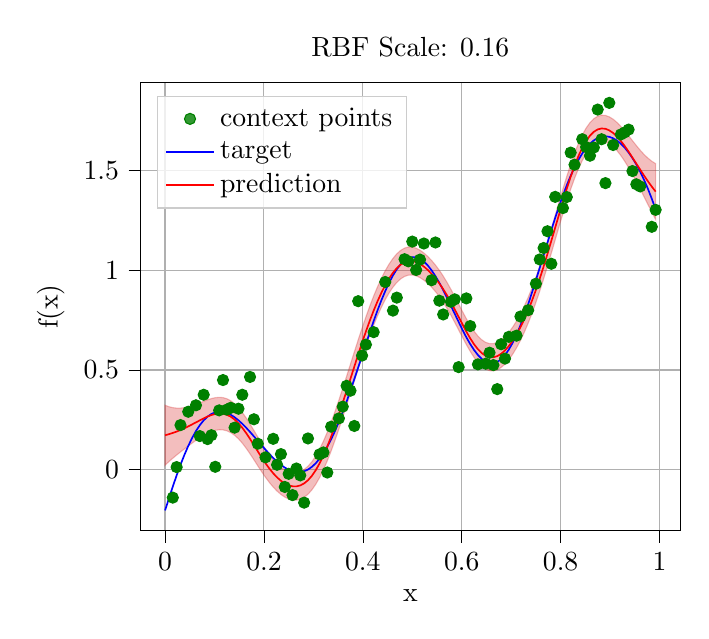
\begin{tikzpicture}

\definecolor{crimson2143940}{RGB}{214,39,40}
\definecolor{darkgray176}{RGB}{176,176,176}
\definecolor{green}{RGB}{0,128,0}
\definecolor{lightgray204}{RGB}{204,204,204}

\begin{axis}[
legend cell align={left},
legend style={
  fill opacity=0.8,
  draw opacity=1,
  text opacity=1,
  at={(0.03,0.97)},
  anchor=north west,
  draw=lightgray204
},
tick align=outside,
tick pos=left,
title={RBF Scale: 0.16},
x grid style={darkgray176},
xlabel={x},
xmajorgrids,
xmin=-0.049609375, xmax=1.041796875,
xtick style={color=black},
y grid style={darkgray176},
ylabel={f(x)},
ymajorgrids,
ymin=-0.307369393110275, ymax=1.94305161833763,
ytick style={color=black}
]
\addplot [draw=green, fill=green, mark=*, only marks]
table{%
x  y
0.015625 -0.140782713890076
0.0234375 0.0124741969630122
0.03125 0.223301634192467
0.046875 0.290305703878403
0.0625 0.322751641273499
0.0703125 0.168172121047974
0.078125 0.375611662864685
0.0859375 0.153029039502144
0.09375 0.172585338354111
0.1015625 0.0139710092917085
0.109375 0.29719278216362
0.1171875 0.449352383613586
0.125 0.30104187130928
0.1328125 0.310201913118362
0.140625 0.210435211658478
0.1484375 0.305497050285339
0.15625 0.375645637512207
0.171875 0.465016812086105
0.1796875 0.252508670091629
0.1875 0.1298718303442
0.203125 0.0613713972270489
0.21875 0.154355853796005
0.2265625 0.0240620393306017
0.234375 0.0776527971029282
0.2421875 -0.087250329554081
0.25 -0.0213457830250263
0.2578125 -0.128125905990601
0.265625 0.00539342686533928
0.2734375 -0.0291735846549273
0.28125 -0.165980145335197
0.2890625 0.15630042552948
0.3125 0.0764417052268982
0.3203125 0.0859965309500694
0.328125 -0.0147307915613055
0.3359375 0.215219244360924
0.3515625 0.256921470165253
0.359375 0.31590062379837
0.3671875 0.420501053333282
0.375 0.395944714546204
0.3828125 0.218961253762245
0.390625 0.845258891582489
0.3984375 0.572290182113647
0.40625 0.627195417881012
0.421875 0.689901649951935
0.4453125 0.941586196422577
0.4609375 0.797937750816345
0.46875 0.863160312175751
0.484375 1.05603492259979
0.4921875 1.04521381855011
0.5 1.14438450336456
0.5078125 1.00189757347107
0.515625 1.05394864082336
0.5234375 1.13475108146667
0.5390625 0.950557947158813
0.546875 1.13994193077087
0.5546875 0.847700536251068
0.5625 0.778648912906647
0.578125 0.842440843582153
0.5859375 0.854452311992645
0.59375 0.514316976070404
0.609375 0.859352290630341
0.6171875 0.720440983772278
0.6328125 0.528135716915131
0.6484375 0.531477034091949
0.65625 0.586675882339478
0.6640625 0.524548232555389
0.671875 0.403894811868668
0.6796875 0.629320204257965
0.6875 0.557079911231995
0.6953125 0.666388988494873
0.7109375 0.672196269035339
0.71875 0.768332600593567
0.734375 0.800018846988678
0.75 0.933004200458527
0.7578125 1.05481159687042
0.765625 1.11214077472687
0.7734375 1.19639194011688
0.78125 1.03309166431427
0.7890625 1.3689421415329
0.8046875 1.31259036064148
0.8125 1.36793231964111
0.8203125 1.59110844135284
0.828125 1.53026258945465
0.84375 1.65839195251465
0.8515625 1.61880052089691
0.859375 1.57554197311401
0.8671875 1.61659646034241
0.875 1.80706143379211
0.8828125 1.65819668769836
0.890625 1.43789076805115
0.8984375 1.84075975418091
0.90625 1.6291788816452
0.921875 1.68228673934937
0.9296875 1.69266092777252
0.9375 1.7065417766571
0.9453125 1.49843001365662
0.953125 1.43219006061554
0.9609375 1.42126441001892
0.984375 1.21854615211487
0.9921875 1.30376839637756
};
\addlegendentry{context points}
\path [draw=crimson2143940, fill=crimson2143940, opacity=0.3]
(axis cs:0,0.322933077812195)
--(axis cs:0,0.0216941684484482)
--(axis cs:0.0078125,0.0398585349321365)
--(axis cs:0.015625,0.0568681359291077)
--(axis cs:0.0234375,0.0729197040200233)
--(axis cs:0.03125,0.0883907675743103)
--(axis cs:0.0390625,0.10344785451889)
--(axis cs:0.046875,0.118173770606518)
--(axis cs:0.0546875,0.132560193538666)
--(axis cs:0.0625,0.146444395184517)
--(axis cs:0.0703125,0.159613281488419)
--(axis cs:0.078125,0.171802878379822)
--(axis cs:0.0859375,0.182492315769196)
--(axis cs:0.09375,0.191118806600571)
--(axis cs:0.1015625,0.197143763303757)
--(axis cs:0.109375,0.19987428188324)
--(axis cs:0.1171875,0.199259579181671)
--(axis cs:0.125,0.194537550210953)
--(axis cs:0.1328125,0.185603022575378)
--(axis cs:0.140625,0.172201439738274)
--(axis cs:0.1484375,0.154316693544388)
--(axis cs:0.15625,0.132626116275787)
--(axis cs:0.1640625,0.107096910476685)
--(axis cs:0.171875,0.0791946649551392)
--(axis cs:0.1796875,0.0493938326835632)
--(axis cs:0.1875,0.0190577954053879)
--(axis cs:0.1953125,-0.0105507075786591)
--(axis cs:0.203125,-0.0387630313634872)
--(axis cs:0.2109375,-0.064655177295208)
--(axis cs:0.21875,-0.0878999605774879)
--(axis cs:0.2265625,-0.108094997704029)
--(axis cs:0.234375,-0.124910540878773)
--(axis cs:0.2421875,-0.138081014156342)
--(axis cs:0.25,-0.147562563419342)
--(axis cs:0.2578125,-0.152811020612717)
--(axis cs:0.265625,-0.153460010886192)
--(axis cs:0.2734375,-0.14909316599369)
--(axis cs:0.28125,-0.139297500252724)
--(axis cs:0.2890625,-0.123723991215229)
--(axis cs:0.296875,-0.10207661986351)
--(axis cs:0.3046875,-0.0743656754493713)
--(axis cs:0.3125,-0.0404715910553932)
--(axis cs:0.3203125,-0.000839486718177795)
--(axis cs:0.328125,0.0439004674553871)
--(axis cs:0.3359375,0.093506321310997)
--(axis cs:0.34375,0.146742433309555)
--(axis cs:0.3515625,0.203184649348259)
--(axis cs:0.359375,0.262140870094299)
--(axis cs:0.3671875,0.32231268286705)
--(axis cs:0.375,0.383164763450623)
--(axis cs:0.3828125,0.444175124168396)
--(axis cs:0.390625,0.504459142684937)
--(axis cs:0.3984375,0.563258290290833)
--(axis cs:0.40625,0.620077192783356)
--(axis cs:0.4140625,0.674043834209442)
--(axis cs:0.421875,0.72469174861908)
--(axis cs:0.4296875,0.771647691726685)
--(axis cs:0.4375,0.81449568271637)
--(axis cs:0.4453125,0.852900862693787)
--(axis cs:0.453125,0.886724650859833)
--(axis cs:0.4609375,0.915639460086823)
--(axis cs:0.46875,0.93919974565506)
--(axis cs:0.4765625,0.957268595695496)
--(axis cs:0.484375,0.96953558921814)
--(axis cs:0.4921875,0.97595226764679)
--(axis cs:0.5,0.976858019828796)
--(axis cs:0.5078125,0.972403228282928)
--(axis cs:0.515625,0.963603854179382)
--(axis cs:0.5234375,0.950779139995575)
--(axis cs:0.53125,0.934753656387329)
--(axis cs:0.5390625,0.915539383888245)
--(axis cs:0.546875,0.893550515174866)
--(axis cs:0.5546875,0.86845725774765)
--(axis cs:0.5625,0.840120553970337)
--(axis cs:0.5703125,0.808868944644928)
--(axis cs:0.578125,0.774738907814026)
--(axis cs:0.5859375,0.738607048988342)
--(axis cs:0.59375,0.701240599155426)
--(axis cs:0.6015625,0.663555145263672)
--(axis cs:0.609375,0.627217054367065)
--(axis cs:0.6171875,0.593374133110046)
--(axis cs:0.625,0.563024938106537)
--(axis cs:0.6328125,0.537693738937378)
--(axis cs:0.640625,0.517834722995758)
--(axis cs:0.6484375,0.504040241241455)
--(axis cs:0.65625,0.496577501296997)
--(axis cs:0.6640625,0.495575785636902)
--(axis cs:0.671875,0.50085312128067)
--(axis cs:0.6796875,0.512355208396912)
--(axis cs:0.6875,0.529403269290924)
--(axis cs:0.6953125,0.551766276359558)
--(axis cs:0.703125,0.579230904579163)
--(axis cs:0.7109375,0.611326932907104)
--(axis cs:0.71875,0.648128092288971)
--(axis cs:0.7265625,0.689276814460754)
--(axis cs:0.734375,0.734904229640961)
--(axis cs:0.7421875,0.784647047519684)
--(axis cs:0.75,0.83856338262558)
--(axis cs:0.7578125,0.896173238754272)
--(axis cs:0.765625,0.957437634468079)
--(axis cs:0.7734375,1.02098953723907)
--(axis cs:0.78125,1.08652901649475)
--(axis cs:0.7890625,1.15330862998962)
--(axis cs:0.796875,1.21974766254425)
--(axis cs:0.8046875,1.28508341312408)
--(axis cs:0.8125,1.34791243076324)
--(axis cs:0.8203125,1.40693283081055)
--(axis cs:0.828125,1.46108388900757)
--(axis cs:0.8359375,1.5093001127243)
--(axis cs:0.84375,1.5506157875061)
--(axis cs:0.8515625,1.58451890945435)
--(axis cs:0.859375,1.61082577705383)
--(axis cs:0.8671875,1.62978100776672)
--(axis cs:0.875,1.64129757881165)
--(axis cs:0.8828125,1.64574790000916)
--(axis cs:0.890625,1.64352071285248)
--(axis cs:0.8984375,1.63485372066498)
--(axis cs:0.90625,1.62049639225006)
--(axis cs:0.9140625,1.60073351860046)
--(axis cs:0.921875,1.57612907886505)
--(axis cs:0.9296875,1.54751396179199)
--(axis cs:0.9375,1.51567876338959)
--(axis cs:0.9453125,1.48103725910187)
--(axis cs:0.953125,1.44491922855377)
--(axis cs:0.9609375,1.4074170589447)
--(axis cs:0.96875,1.3694087266922)
--(axis cs:0.9765625,1.33117532730103)
--(axis cs:0.984375,1.29296278953552)
--(axis cs:0.9921875,1.25516641139984)
--(axis cs:0.9921875,1.53571736812592)
--(axis cs:0.9921875,1.53571736812592)
--(axis cs:0.984375,1.54791283607483)
--(axis cs:0.9765625,1.56342267990112)
--(axis cs:0.96875,1.58198845386505)
--(axis cs:0.9609375,1.60316896438599)
--(axis cs:0.953125,1.62659060955048)
--(axis cs:0.9453125,1.65103662014008)
--(axis cs:0.9375,1.67607057094574)
--(axis cs:0.9296875,1.70012617111206)
--(axis cs:0.921875,1.7225729227066)
--(axis cs:0.9140625,1.74242758750916)
--(axis cs:0.90625,1.75868737697601)
--(axis cs:0.8984375,1.77061140537262)
--(axis cs:0.890625,1.77767622470856)
--(axis cs:0.8828125,1.77884554862976)
--(axis cs:0.875,1.77361631393433)
--(axis cs:0.8671875,1.76134777069092)
--(axis cs:0.859375,1.74153184890747)
--(axis cs:0.8515625,1.71420288085938)
--(axis cs:0.84375,1.67917156219482)
--(axis cs:0.8359375,1.63668167591095)
--(axis cs:0.828125,1.58734822273254)
--(axis cs:0.8203125,1.53214001655579)
--(axis cs:0.8125,1.47223103046417)
--(axis cs:0.8046875,1.40869605541229)
--(axis cs:0.796875,1.34284698963165)
--(axis cs:0.7890625,1.27614760398865)
--(axis cs:0.78125,1.20937585830688)
--(axis cs:0.7734375,1.14413940906525)
--(axis cs:0.765625,1.08122384548187)
--(axis cs:0.7578125,1.0209242105484)
--(axis cs:0.75,0.964600503444672)
--(axis cs:0.7421875,0.912259161472321)
--(axis cs:0.734375,0.864302217960358)
--(axis cs:0.7265625,0.820542454719543)
--(axis cs:0.71875,0.781222283840179)
--(axis cs:0.7109375,0.746068120002747)
--(axis cs:0.703125,0.715322613716125)
--(axis cs:0.6953125,0.688788890838623)
--(axis cs:0.6875,0.666898190975189)
--(axis cs:0.6796875,0.649891138076782)
--(axis cs:0.671875,0.63801497220993)
--(axis cs:0.6640625,0.632050275802612)
--(axis cs:0.65625,0.632128000259399)
--(axis cs:0.6484375,0.638545274734497)
--(axis cs:0.640625,0.651264846324921)
--(axis cs:0.6328125,0.670093178749084)
--(axis cs:0.625,0.694499313831329)
--(axis cs:0.6171875,0.724108695983887)
--(axis cs:0.609375,0.757389545440674)
--(axis cs:0.6015625,0.793396949768066)
--(axis cs:0.59375,0.831000864505768)
--(axis cs:0.5859375,0.868505716323853)
--(axis cs:0.578125,0.904996633529663)
--(axis cs:0.5703125,0.939653217792511)
--(axis cs:0.5625,0.971588492393494)
--(axis cs:0.5546875,1.00072503089905)
--(axis cs:0.546875,1.02672100067139)
--(axis cs:0.5390625,1.04970526695251)
--(axis cs:0.53125,1.07000708580017)
--(axis cs:0.5234375,1.08720147609711)
--(axis cs:0.515625,1.10125601291656)
--(axis cs:0.5078125,1.11130952835083)
--(axis cs:0.5,1.11698567867279)
--(axis cs:0.4921875,1.11721456050873)
--(axis cs:0.484375,1.11181259155273)
--(axis cs:0.4765625,1.10040175914764)
--(axis cs:0.46875,1.08301568031311)
--(axis cs:0.4609375,1.06002628803253)
--(axis cs:0.453125,1.0315682888031)
--(axis cs:0.4453125,0.998133420944214)
--(axis cs:0.4375,0.960091590881348)
--(axis cs:0.4296875,0.917578339576721)
--(axis cs:0.421875,0.870932817459106)
--(axis cs:0.4140625,0.820523917675018)
--(axis cs:0.40625,0.766732037067413)
--(axis cs:0.3984375,0.709992289543152)
--(axis cs:0.390625,0.651187062263489)
--(axis cs:0.3828125,0.590782284736633)
--(axis cs:0.375,0.529563307762146)
--(axis cs:0.3671875,0.468413859605789)
--(axis cs:0.359375,0.407886624336243)
--(axis cs:0.3515625,0.348519384860992)
--(axis cs:0.34375,0.291622519493103)
--(axis cs:0.3359375,0.237886890769005)
--(axis cs:0.328125,0.187743782997131)
--(axis cs:0.3203125,0.142417952418327)
--(axis cs:0.3125,0.102153368294239)
--(axis cs:0.3046875,0.0675596594810486)
--(axis cs:0.296875,0.0391018390655518)
--(axis cs:0.2890625,0.0166653022170067)
--(axis cs:0.28125,0.000308647751808167)
--(axis cs:0.2734375,-0.0102628618478775)
--(axis cs:0.265625,-0.0153135359287262)
--(axis cs:0.2578125,-0.0152201578021049)
--(axis cs:0.25,-0.0103302076458931)
--(axis cs:0.2421875,-0.000947542488574982)
--(axis cs:0.234375,0.0124079361557961)
--(axis cs:0.2265625,0.0297127440571785)
--(axis cs:0.21875,0.0507357195019722)
--(axis cs:0.2109375,0.0751478597521782)
--(axis cs:0.203125,0.102511450648308)
--(axis cs:0.1953125,0.132486641407013)
--(axis cs:0.1875,0.16411118209362)
--(axis cs:0.1796875,0.19666776061058)
--(axis cs:0.171875,0.228811293840408)
--(axis cs:0.1640625,0.259116381406784)
--(axis cs:0.15625,0.286974042654037)
--(axis cs:0.1484375,0.310832977294922)
--(axis cs:0.140625,0.330595672130585)
--(axis cs:0.1328125,0.345534682273865)
--(axis cs:0.125,0.355660170316696)
--(axis cs:0.1171875,0.361283719539642)
--(axis cs:0.109375,0.362710952758789)
--(axis cs:0.1015625,0.360984116792679)
--(axis cs:0.09375,0.356439858675003)
--(axis cs:0.0859375,0.350048243999481)
--(axis cs:0.078125,0.342566251754761)
--(axis cs:0.0703125,0.334760069847107)
--(axis cs:0.0625,0.32728385925293)
--(axis cs:0.0546875,0.320548802614212)
--(axis cs:0.046875,0.314937263727188)
--(axis cs:0.0390625,0.310870677232742)
--(axis cs:0.03125,0.308645874261856)
--(axis cs:0.0234375,0.308583855628967)
--(axis cs:0.015625,0.31084731221199)
--(axis cs:0.0078125,0.315595865249634)
--(axis cs:0,0.322933077812195)
--cycle;

\addplot [semithick, blue]
table {%
0 -0.205077528953552
0.015625 -0.0854612588882446
0.0234375 -0.0290179252624512
0.03125 0.0241776704788208
0.0390625 0.073489785194397
0.046875 0.118387222290039
0.0546875 0.158448100090027
0.0625 0.193363189697266
0.0703125 0.222933530807495
0.078125 0.247067928314209
0.0859375 0.265776634216309
0.09375 0.279163122177124
0.1015625 0.287414908409119
0.109375 0.29079258441925
0.1171875 0.289618492126465
0.125 0.284265160560608
0.1328125 0.275144934654236
0.140625 0.262698769569397
0.1484375 0.247387528419495
0.15625 0.229683041572571
0.1640625 0.210062503814697
0.171875 0.18900191783905
0.1875 0.144443511962891
0.203125 0.0996959209442139
0.2109375 0.0783662796020508
0.21875 0.0583091974258423
0.2265625 0.0399456024169922
0.234375 0.0236865282058716
0.2421875 0.00993156433105469
0.25 -0.000932693481445312
0.2578125 -0.00853729248046875
0.265625 -0.012534499168396
0.2734375 -0.0126035213470459
0.28125 -0.00845754146575928
0.2890625 0.000149250030517578
0.296875 0.0134142637252808
0.3046875 0.0314778089523315
0.3125 0.0544165372848511
0.3203125 0.0822352170944214
0.328125 0.114861488342285
0.3359375 0.152141571044922
0.34375 0.193836569786072
0.3515625 0.239622235298157
0.359375 0.289090037345886
0.3671875 0.341750860214233
0.375 0.397040486335754
0.390625 0.512924909591675
0.4140625 0.689096927642822
0.421875 0.745354175567627
0.4296875 0.79908299446106
0.4375 0.84954047203064
0.4453125 0.896026849746704
0.453125 0.937900066375732
0.4609375 0.974589467048645
0.46875 1.00560748577118
0.4765625 1.03056013584137
0.484375 1.04915428161621
0.4921875 1.06120634078979
0.5 1.06664550304413
0.5078125 1.06551682949066
0.515625 1.05798196792603
0.5234375 1.04431772232056
0.53125 1.02491223812103
0.5390625 1.00026059150696
0.546875 0.970956087112427
0.5546875 0.937681794166565
0.5625 0.901200532913208
0.5703125 0.862339973449707
0.6015625 0.701167941093445
0.609375 0.664103269577026
0.6171875 0.630154848098755
0.625 0.600165247917175
0.6328125 0.574909210205078
0.640625 0.555077791213989
0.6484375 0.541262149810791
0.65625 0.533941745758057
0.6640625 0.53347373008728
0.671875 0.540083169937134
0.6796875 0.55385947227478
0.6875 0.574752807617188
0.6953125 0.602575778961182
0.703125 0.637008666992188
0.7109375 0.677605152130127
0.71875 0.723804950714111
0.7265625 0.774946093559265
0.734375 0.830281734466553
0.7421875 0.88899827003479
0.7578125 1.01309990882874
0.78125 1.20261490345001
0.7890625 1.26327884197235
0.796875 1.32141351699829
0.8046875 1.37636232376099
0.8125 1.4275563955307
0.8203125 1.47452008724213
0.828125 1.51687347888947
0.8359375 1.55433392524719
0.84375 1.586709856987
0.8515625 1.61389589309692
0.859375 1.63586342334747
0.8671875 1.65264868736267
0.875 1.66434049606323
0.8828125 1.6710661649704
0.890625 1.67297780513763
0.8984375 1.67023825645447
0.90625 1.66300654411316
0.9140625 1.65142905712128
0.921875 1.63562655448914
0.9296875 1.61568832397461
0.9375 1.59166574478149
0.9453125 1.56356978416443
0.953125 1.53137040138245
0.9609375 1.49499881267548
0.96875 1.45435214042664
0.9765625 1.40929961204529
0.984375 1.35969078540802
0.9921875 1.30536472797394
};
\addlegendentry{target}
\addplot [semithick, red]
table {%
0 0.172313570976257
0.0078125 0.177727222442627
0.015625 0.183857679367065
0.0234375 0.190751791000366
0.03125 0.1985182762146
0.0390625 0.207159280776978
0.046875 0.21655547618866
0.0625 0.23686408996582
0.078125 0.257184505462646
0.0859375 0.266270279884338
0.09375 0.273779392242432
0.1015625 0.279063940048218
0.109375 0.281292676925659
0.1171875 0.280271649360657
0.125 0.27509880065918
0.1328125 0.265568852424622
0.140625 0.25139856338501
0.1484375 0.232574820518494
0.15625 0.209800124168396
0.1640625 0.183106660842896
0.171875 0.154003024101257
0.1953125 0.0609679222106934
0.203125 0.0318741798400879
0.2109375 0.00524640083312988
0.21875 -0.0185821056365967
0.2265625 -0.0391911268234253
0.234375 -0.0562512874603271
0.2421875 -0.069514274597168
0.25 -0.0789463520050049
0.2578125 -0.0840156078338623
0.265625 -0.0843868255615234
0.2734375 -0.0796780586242676
0.28125 -0.0694944858551025
0.2890625 -0.0535293817520142
0.296875 -0.0314873456954956
0.3046875 -0.0034029483795166
0.3125 0.0308408737182617
0.3203125 0.0707892179489136
0.328125 0.115822076797485
0.3359375 0.165696620941162
0.34375 0.21918249130249
0.3515625 0.275851964950562
0.3671875 0.395363330841064
0.390625 0.577823162078857
0.3984375 0.636625289916992
0.40625 0.693404674530029
0.4140625 0.747283935546875
0.421875 0.797812223434448
0.4296875 0.844613075256348
0.4375 0.887293577194214
0.4453125 0.925517082214355
0.453125 0.959146499633789
0.4609375 0.98783278465271
0.46875 1.01110768318176
0.4765625 1.02883517742157
0.484375 1.04067409038544
0.4921875 1.04658341407776
0.5 1.04692184925079
0.5078125 1.0418564081192
0.515625 1.03242993354797
0.5234375 1.01899027824402
0.53125 1.00238037109375
0.5390625 0.982622385025024
0.546875 0.960135698318481
0.5546875 0.934591054916382
0.5625 0.905854463577271
0.5703125 0.874261140823364
0.578125 0.839867830276489
0.5859375 0.803556442260742
0.609375 0.69230329990387
0.6171875 0.658741474151611
0.625 0.628762125968933
0.6328125 0.603893518447876
0.640625 0.584549784660339
0.6484375 0.571292757987976
0.65625 0.564352750778198
0.6640625 0.563812971115112
0.671875 0.5694340467453
0.6796875 0.581123113632202
0.6875 0.598150730133057
0.6953125 0.620277643203735
0.703125 0.647276759147644
0.7109375 0.67869758605957
0.71875 0.714675188064575
0.7265625 0.754909634590149
0.734375 0.799603223800659
0.7421875 0.848453044891357
0.75 0.901582002639771
0.7578125 0.958548784255981
0.765625 1.01933073997498
0.7734375 1.08256447315216
0.7890625 1.21472811698914
0.8046875 1.34688973426819
0.8125 1.41007173061371
0.8203125 1.46953642368317
0.828125 1.52421605587006
0.8359375 1.57299089431763
0.84375 1.61489367485046
0.8515625 1.64936089515686
0.859375 1.67617881298065
0.8671875 1.69556438922882
0.875 1.70745694637299
0.8828125 1.71229672431946
0.890625 1.71059846878052
0.8984375 1.7027325630188
0.90625 1.68959188461304
0.9140625 1.67158055305481
0.921875 1.64935100078583
0.9296875 1.62382006645203
0.9375 1.59587466716766
0.953125 1.53575491905212
0.96875 1.47569859027863
0.9765625 1.44729900360107
0.984375 1.42043781280518
0.9921875 1.39544188976288
};
\addlegendentry{prediction}
\end{axis}

\end{tikzpicture}

	}
	\caption{Model A prediction plots with increasing number of context points (5,10,50).}
	\label{fig:result_plot}
\end{figure*}

For all models, we observe increasing performance with an increasing number of context points. This is clearly visible in \autoref{fig:result_plot}, with the left and middle plots showing a lot of uncertainty due to the low number of context points. The right plot shows the prediction much closer to the target despite a large amount of noise. Furthermore, evaluations on the Version-B datasets show better performance than evaluations on Version-A datasets. This is expected as Dataset-A is more challenging. Model-B showing similar performance to Model-A on Dataset-A, despite being trained on the less challenging Dataset-B, might be sign of good generalization capabilities. However, as shown in \autoref{fig:beta_scales}, the RBF-Scale distributions show a large overlap. For this reason, Model-B has seen sufficient examples of challenging functions during training and the similar performance cannot be attributed to generalization.

\begin{figure}
	\centering
	\resizebox{0.5\textwidth}{!}{
		% This file was created with matplot2tikz v0.4.0.
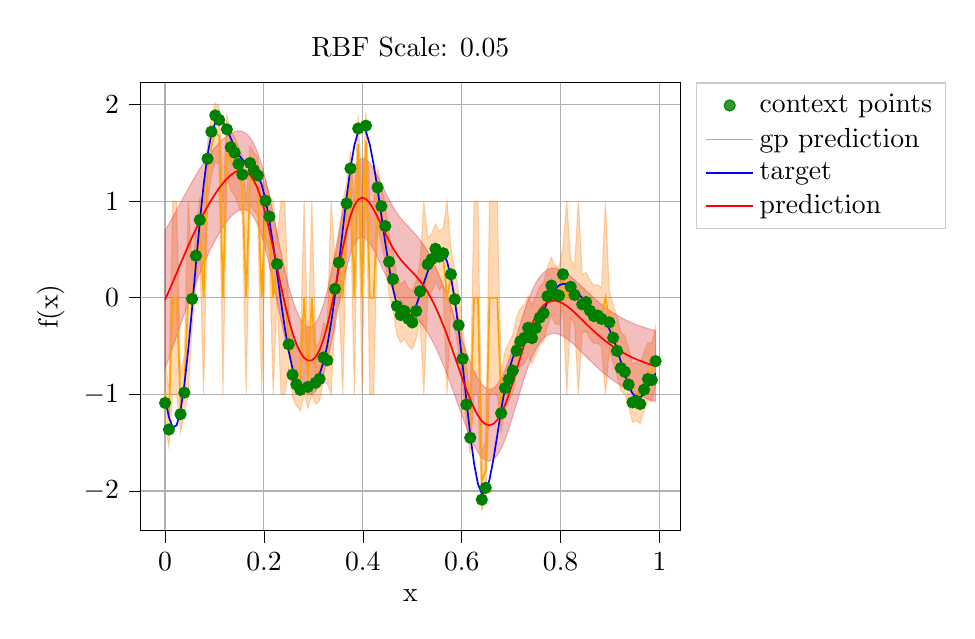
\begin{tikzpicture}

\definecolor{crimson2143940}{RGB}{214,39,40}
\definecolor{darkgray176}{RGB}{176,176,176}
\definecolor{darkorange25512714}{RGB}{255,127,14}
\definecolor{green}{RGB}{0,128,0}
\definecolor{lightgray204}{RGB}{204,204,204}
\definecolor{orange}{RGB}{255,165,0}

\begin{axis}[
legend pos=outer north east,
legend cell align={left},
legend style={fill opacity=0.8, draw opacity=1, text opacity=1, draw=lightgray204},
tick align=outside,
tick pos=left,
title={RBF Scale: 0.05},
x grid style={darkgray176},
xlabel={x},
xmajorgrids,
xmin=-0.049609375, xmax=1.041796875,
xtick style={color=black},
y grid style={darkgray176},
ylabel={f(x)},
ymajorgrids,
ymin=-2.41224553995949, ymax=2.22731967114439,
ytick style={color=black}
]
\path [draw=darkorange25512714, fill=darkorange25512714, opacity=0.3]
(axis cs:0,-0.688383328985389)
--(axis cs:0,-1.29140601814092)
--(axis cs:0.0078125,-1.5413831705177)
--(axis cs:0.015625,-1)
--(axis cs:0.0234375,-1)
--(axis cs:0.03125,-1.39722157817871)
--(axis cs:0.0390625,-1.19397662668188)
--(axis cs:0.046875,-1)
--(axis cs:0.0546875,-0.312615969509551)
--(axis cs:0.0625,0.0932374694935545)
--(axis cs:0.0703125,0.430423814398134)
--(axis cs:0.078125,-1)
--(axis cs:0.0859375,1.00660140596913)
--(axis cs:0.09375,1.26045424831494)
--(axis cs:0.1015625,1.41340765421142)
--(axis cs:0.109375,1.37199936832405)
--(axis cs:0.1171875,-1)
--(axis cs:0.125,1.28255494331056)
--(axis cs:0.1328125,1.11365753849997)
--(axis cs:0.140625,1.06352678776651)
--(axis cs:0.1484375,0.956532171873315)
--(axis cs:0.15625,0.856964259341907)
--(axis cs:0.1640625,-1)
--(axis cs:0.171875,0.965423036921057)
--(axis cs:0.1796875,0.89815274910732)
--(axis cs:0.1875,0.8489957996014)
--(axis cs:0.1953125,-1)
--(axis cs:0.203125,0.610918073287938)
--(axis cs:0.2109375,0.461912394270764)
--(axis cs:0.21875,-1)
--(axis cs:0.2265625,0.0152650413264633)
--(axis cs:0.234375,-1)
--(axis cs:0.2421875,-1)
--(axis cs:0.25,-0.740297259312786)
--(axis cs:0.2578125,-1.02614532124722)
--(axis cs:0.265625,-1.11755500873782)
--(axis cs:0.2734375,-1.16809834347397)
--(axis cs:0.28125,-1)
--(axis cs:0.2890625,-1.13998389361326)
--(axis cs:0.296875,-1)
--(axis cs:0.3046875,-1.10139643136165)
--(axis cs:0.3125,-1.06571634374099)
--(axis cs:0.3203125,-0.863651326395437)
--(axis cs:0.328125,-0.890382622091687)
--(axis cs:0.3359375,-1)
--(axis cs:0.34375,-0.218288157083889)
--(axis cs:0.3515625,0.0299163128477336)
--(axis cs:0.359375,-1)
--(axis cs:0.3671875,0.584659180134388)
--(axis cs:0.375,0.915193592947601)
--(axis cs:0.3828125,-1)
--(axis cs:0.390625,1.290893798502)
--(axis cs:0.3984375,-1)
--(axis cs:0.40625,1.31714457989889)
--(axis cs:0.4140625,-1)
--(axis cs:0.421875,-1)
--(axis cs:0.4296875,0.735886932895363)
--(axis cs:0.4375,0.559125384839859)
--(axis cs:0.4453125,0.371735822723044)
--(axis cs:0.453125,0.0368862627547937)
--(axis cs:0.4609375,-0.127295112219921)
--(axis cs:0.46875,-0.378900165420577)
--(axis cs:0.4765625,-0.464845701930011)
--(axis cs:0.484375,-0.426493428332804)
--(axis cs:0.4921875,-0.50154131099667)
--(axis cs:0.5,-0.534409846037235)
--(axis cs:0.5078125,-0.426543569491712)
--(axis cs:0.515625,-0.241967819964512)
--(axis cs:0.5234375,-1)
--(axis cs:0.53125,0.0122248665430005)
--(axis cs:0.5390625,0.0602919132122145)
--(axis cs:0.546875,0.158896214718978)
--(axis cs:0.5546875,0.0846877741175106)
--(axis cs:0.5625,0.116868292496573)
--(axis cs:0.5703125,-1)
--(axis cs:0.578125,-0.0813338984325448)
--(axis cs:0.5859375,-0.316384265851202)
--(axis cs:0.59375,-0.560231258330496)
--(axis cs:0.6015625,-0.876462848827993)
--(axis cs:0.609375,-1.30663025659162)
--(axis cs:0.6171875,-1.61851670489081)
--(axis cs:0.625,-1)
--(axis cs:0.6328125,-1)
--(axis cs:0.640625,-2.20135621218204)
--(axis cs:0.6484375,-2.08992262848657)
--(axis cs:0.65625,-1)
--(axis cs:0.6640625,-1)
--(axis cs:0.671875,-1)
--(axis cs:0.6796875,-1.38823123426756)
--(axis cs:0.6875,-1.15162244906953)
--(axis cs:0.6953125,-1.06873940030507)
--(axis cs:0.703125,-0.987399313245003)
--(axis cs:0.7109375,-0.800413053019892)
--(axis cs:0.71875,-0.711758029811619)
--(axis cs:0.7265625,-0.679632507817893)
--(axis cs:0.734375,-0.583887351931207)
--(axis cs:0.7421875,-0.681631199463245)
--(axis cs:0.75,-0.584985494806654)
--(axis cs:0.7578125,-0.488159440646371)
--(axis cs:0.765625,-0.447267140033861)
--(axis cs:0.7734375,-0.287496374950949)
--(axis cs:0.78125,-0.186992655461015)
--(axis cs:0.7890625,-0.269502708169921)
--(axis cs:0.796875,-0.281603215293504)
--(axis cs:0.8046875,-0.0812010894034952)
--(axis cs:0.8125,-1)
--(axis cs:0.8203125,-0.198774182942497)
--(axis cs:0.828125,-0.275112009113055)
--(axis cs:0.8359375,-1)
--(axis cs:0.84375,-0.363647653058834)
--(axis cs:0.8515625,-0.34228646896296)
--(axis cs:0.859375,-0.423369229554881)
--(axis cs:0.8671875,-0.474572072217907)
--(axis cs:0.875,-0.469278532642914)
--(axis cs:0.8828125,-0.500621643663753)
--(axis cs:0.890625,-1)
--(axis cs:0.8984375,-0.53333254879791)
--(axis cs:0.90625,-0.677590134405544)
--(axis cs:0.9140625,-0.801608029662508)
--(axis cs:0.921875,-0.963462625849322)
--(axis cs:0.9296875,-0.998288812851843)
--(axis cs:0.9375,-1.1192513280054)
--(axis cs:0.9453125,-1.2865681735166)
--(axis cs:0.953125,-1.27205635452423)
--(axis cs:0.9609375,-1.3019123402926)
--(axis cs:0.96875,-1.16662625583365)
--(axis cs:0.9765625,-1.06622264929502)
--(axis cs:0.984375,-1.07593145893693)
--(axis cs:0.9921875,-0.898316631155426)
--(axis cs:0.9921875,-0.295293941999899)
--(axis cs:0.9921875,-0.295293941999899)
--(axis cs:0.984375,-0.472908769781403)
--(axis cs:0.9765625,-0.463199960139497)
--(axis cs:0.96875,-0.563603566678123)
--(axis cs:0.9609375,-0.698889651137071)
--(axis cs:0.953125,-0.669033665368699)
--(axis cs:0.9453125,-0.683545484361075)
--(axis cs:0.9375,-0.516228638849877)
--(axis cs:0.9296875,-0.395266123696316)
--(axis cs:0.921875,-0.360439936693794)
--(axis cs:0.9140625,-0.19858534050698)
--(axis cs:0.90625,-0.0745674452500167)
--(axis cs:0.8984375,0.0696901403576179)
--(axis cs:0.890625,1)
--(axis cs:0.8828125,0.102401045491775)
--(axis cs:0.875,0.133744156512613)
--(axis cs:0.8671875,0.12845061693762)
--(axis cs:0.859375,0.179653459600647)
--(axis cs:0.8515625,0.260736220192568)
--(axis cs:0.84375,0.239375036096694)
--(axis cs:0.8359375,1)
--(axis cs:0.828125,0.327910680042473)
--(axis cs:0.8203125,0.404248506213031)
--(axis cs:0.8125,1)
--(axis cs:0.8046875,0.521821599752032)
--(axis cs:0.796875,0.321419473862024)
--(axis cs:0.7890625,0.333519980985607)
--(axis cs:0.78125,0.416030033694513)
--(axis cs:0.7734375,0.315526314204578)
--(axis cs:0.765625,0.155755549121667)
--(axis cs:0.7578125,0.114863248509157)
--(axis cs:0.75,0.0180371943488732)
--(axis cs:0.7421875,-0.0786085103077172)
--(axis cs:0.734375,0.0191353372243203)
--(axis cs:0.7265625,-0.0766098186623656)
--(axis cs:0.71875,-0.108735340656092)
--(axis cs:0.7109375,-0.197390363864365)
--(axis cs:0.703125,-0.384376624089476)
--(axis cs:0.6953125,-0.465716711149538)
--(axis cs:0.6875,-0.548599759914007)
--(axis cs:0.6796875,-0.785208545112036)
--(axis cs:0.671875,1)
--(axis cs:0.6640625,1)
--(axis cs:0.65625,1)
--(axis cs:0.6484375,-1.48689993933105)
--(axis cs:0.640625,-1.59833352302651)
--(axis cs:0.6328125,1)
--(axis cs:0.625,1)
--(axis cs:0.6171875,-1.01549401573528)
--(axis cs:0.609375,-0.70360756743609)
--(axis cs:0.6015625,-0.273440159672465)
--(axis cs:0.59375,0.0427914308250313)
--(axis cs:0.5859375,0.286638423304326)
--(axis cs:0.578125,0.521688790722983)
--(axis cs:0.5703125,1)
--(axis cs:0.5625,0.719890981652101)
--(axis cs:0.5546875,0.687710463273038)
--(axis cs:0.546875,0.761918903874506)
--(axis cs:0.5390625,0.663314602367742)
--(axis cs:0.53125,0.615247555698528)
--(axis cs:0.5234375,1)
--(axis cs:0.515625,0.361054869191016)
--(axis cs:0.5078125,0.176479119663816)
--(axis cs:0.5,0.0686128431182931)
--(axis cs:0.4921875,0.101481378158857)
--(axis cs:0.484375,0.176529260822724)
--(axis cs:0.4765625,0.138176987225517)
--(axis cs:0.46875,0.224122523734951)
--(axis cs:0.4609375,0.475727576935606)
--(axis cs:0.453125,0.639908951910321)
--(axis cs:0.4453125,0.974758511878572)
--(axis cs:0.4375,1.16214807399539)
--(axis cs:0.4296875,1.33890962205089)
--(axis cs:0.421875,1)
--(axis cs:0.4140625,1)
--(axis cs:0.40625,1.92016726905442)
--(axis cs:0.3984375,1)
--(axis cs:0.390625,1.89391648765753)
--(axis cs:0.3828125,1)
--(axis cs:0.375,1.51821628210313)
--(axis cs:0.3671875,1.18768186928992)
--(axis cs:0.359375,1)
--(axis cs:0.3515625,0.632939002003261)
--(axis cs:0.34375,0.384734532071639)
--(axis cs:0.3359375,1)
--(axis cs:0.328125,-0.287359932936159)
--(axis cs:0.3203125,-0.260628637239909)
--(axis cs:0.3125,-0.462693654585458)
--(axis cs:0.3046875,-0.498373742206126)
--(axis cs:0.296875,1)
--(axis cs:0.2890625,-0.536961204457736)
--(axis cs:0.28125,1)
--(axis cs:0.2734375,-0.565075654318443)
--(axis cs:0.265625,-0.514532319582289)
--(axis cs:0.2578125,-0.423122632091688)
--(axis cs:0.25,-0.137274570157258)
--(axis cs:0.2421875,1)
--(axis cs:0.234375,1)
--(axis cs:0.2265625,0.618287730481991)
--(axis cs:0.21875,1)
--(axis cs:0.2109375,1.06493508342629)
--(axis cs:0.203125,1.21394076244347)
--(axis cs:0.1953125,1)
--(axis cs:0.1875,1.45201848875693)
--(axis cs:0.1796875,1.50117543826285)
--(axis cs:0.171875,1.56844572607658)
--(axis cs:0.1640625,1)
--(axis cs:0.15625,1.45998694849743)
--(axis cs:0.1484375,1.55955486102884)
--(axis cs:0.140625,1.66654947692204)
--(axis cs:0.1328125,1.7166802276555)
--(axis cs:0.125,1.88557763246609)
--(axis cs:0.1171875,1)
--(axis cs:0.109375,1.97502205747958)
--(axis cs:0.1015625,2.01643034336694)
--(axis cs:0.09375,1.86347693747047)
--(axis cs:0.0859375,1.60962409512466)
--(axis cs:0.078125,1)
--(axis cs:0.0703125,1.03344650355366)
--(axis cs:0.0625,0.696260158649082)
--(axis cs:0.0546875,0.290406719645977)
--(axis cs:0.046875,1)
--(axis cs:0.0390625,-0.590953937526351)
--(axis cs:0.03125,-0.794198889023184)
--(axis cs:0.0234375,1)
--(axis cs:0.015625,1)
--(axis cs:0.0078125,-0.938360481362176)
--(axis cs:0,-0.688383328985389)
--cycle;

\addplot [draw=green, fill=green, mark=*, only marks]
table{%
x  y
0 -1.08888411521912
0.0078125 -1.36385905742645
0.03125 -1.20528125762939
0.0390625 -0.981711804866791
0.0546875 -0.0122150871902704
0.0625 0.434223681688309
0.0703125 0.805128693580627
0.0859375 1.43892407417297
0.09375 1.71816217899323
0.1015625 1.88641095161438
0.109375 1.84086179733276
0.125 1.74247288703918
0.1328125 1.55668580532074
0.140625 1.50154197216034
0.1484375 1.38384783267975
0.15625 1.27432310581207
0.171875 1.39362776279449
0.1796875 1.31963050365448
0.1875 1.26555788516998
0.203125 1.0036723613739
0.2109375 0.839766085147858
0.2265625 0.348454028367996
0.25 -0.482664495706558
0.2578125 -0.797097384929657
0.265625 -0.89764803647995
0.2734375 -0.95324569940567
0.2890625 -0.922319829463959
0.3046875 -0.87987357378006
0.3125 -0.840625524520874
0.3203125 -0.618353962898254
0.328125 -0.647758424282074
0.34375 0.091545507311821
0.3515625 0.364570409059525
0.3671875 0.974787592887878
0.375 1.3383754491806
0.390625 1.75164568424225
0.40625 1.78052151203156
0.4296875 1.14113807678223
0.4375 0.946700394153595
0.4453125 0.740571856498718
0.453125 0.372237354516983
0.4609375 0.191637858748436
0.46875 -0.0851277038455009
0.4765625 -0.179667785763741
0.484375 -0.137480288743973
0.4921875 -0.220032960176468
0.5 -0.256188362836838
0.5078125 -0.137535452842712
0.515625 0.065497875213623
0.53125 0.345109820365906
0.5390625 0.397983580827713
0.546875 0.506448328495026
0.5546875 0.424819022417068
0.5625 0.460217595100403
0.578125 0.242195188999176
0.5859375 -0.0163602139800787
0.59375 -0.284591913223267
0.6015625 -0.632446646690369
0.609375 -1.1056307554245
0.6171875 -1.44870591163635
0.640625 -2.08982944488525
0.6484375 -1.96725237369537
0.6796875 -1.19539189338684
0.6875 -0.935122191905975
0.6953125 -0.843950867652893
0.703125 -0.75447678565979
0.7109375 -0.548791885375977
0.71875 -0.45127135515213
0.7265625 -0.415933281183243
0.734375 -0.310613602399826
0.7421875 -0.418131828308105
0.75 -0.311821579933167
0.7578125 -0.20531290769577
0.765625 -0.16033136844635
0.7734375 0.0154164666309953
0.78125 0.125970557332039
0.7890625 0.0352094992995262
0.796875 0.0218989420682192
0.8046875 0.242341279983521
0.8203125 0.113010875880718
0.828125 0.0290392693132162
0.84375 -0.0683499425649643
0.8515625 -0.0448526367545128
0.859375 -0.134043678641319
0.8671875 -0.190366804599762
0.875 -0.184543907642365
0.8828125 -0.219021335244179
0.8984375 -0.255003333091736
0.90625 -0.413686662912369
0.9140625 -0.550106346607208
0.921875 -0.728146433830261
0.9296875 -0.766455233097076
0.9375 -0.899513959884644
0.9453125 -1.08356249332428
0.953125 -1.0675995349884
0.9609375 -1.1004410982132
0.96875 -0.951626420021057
0.9765625 -0.84118241071701
0.984375 -0.851862132549286
0.9921875 -0.656485795974731
};
\addlegendentry{context points}
\path [draw=crimson2143940, fill=crimson2143940, opacity=0.3]
(axis cs:0,0.696671664714813)
--(axis cs:0,-0.740054786205292)
--(axis cs:0.0078125,-0.627373278141022)
--(axis cs:0.015625,-0.512808382511139)
--(axis cs:0.0234375,-0.39756977558136)
--(axis cs:0.03125,-0.282166302204132)
--(axis cs:0.0390625,-0.168199002742767)
--(axis cs:0.046875,-0.0565215349197388)
--(axis cs:0.0546875,0.0512517094612122)
--(axis cs:0.0625,0.154866576194763)
--(axis cs:0.0703125,0.253698348999023)
--(axis cs:0.078125,0.347421884536743)
--(axis cs:0.0859375,0.435442745685577)
--(axis cs:0.09375,0.518145859241486)
--(axis cs:0.1015625,0.595096349716187)
--(axis cs:0.109375,0.666191160678864)
--(axis cs:0.1171875,0.730400323867798)
--(axis cs:0.125,0.787310838699341)
--(axis cs:0.1328125,0.836141228675842)
--(axis cs:0.140625,0.874897301197052)
--(axis cs:0.1484375,0.901703417301178)
--(axis cs:0.15625,0.914355278015137)
--(axis cs:0.1640625,0.909058213233948)
--(axis cs:0.171875,0.882757663726807)
--(axis cs:0.1796875,0.831635653972626)
--(axis cs:0.1875,0.752900958061218)
--(axis cs:0.1953125,0.643742799758911)
--(axis cs:0.203125,0.504491329193115)
--(axis cs:0.2109375,0.339611321687698)
--(axis cs:0.21875,0.155899345874786)
--(axis cs:0.2265625,-0.0371500253677368)
--(axis cs:0.234375,-0.227965235710144)
--(axis cs:0.2421875,-0.408678412437439)
--(axis cs:0.25,-0.571097910404205)
--(axis cs:0.2578125,-0.709887862205505)
--(axis cs:0.265625,-0.823691725730896)
--(axis cs:0.2734375,-0.910091876983643)
--(axis cs:0.28125,-0.969185590744019)
--(axis cs:0.2890625,-0.998992562294006)
--(axis cs:0.296875,-0.99879515171051)
--(axis cs:0.3046875,-0.965435385704041)
--(axis cs:0.3125,-0.897048354148865)
--(axis cs:0.3203125,-0.791982352733612)
--(axis cs:0.328125,-0.651382267475128)
--(axis cs:0.3359375,-0.477786332368851)
--(axis cs:0.34375,-0.281131595373154)
--(axis cs:0.3515625,-0.0732633173465729)
--(axis cs:0.359375,0.129022240638733)
--(axis cs:0.3671875,0.309002429246902)
--(axis cs:0.375,0.453575879335403)
--(axis cs:0.3828125,0.555606245994568)
--(axis cs:0.390625,0.613325834274292)
--(axis cs:0.3984375,0.62926185131073)
--(axis cs:0.40625,0.61024135351181)
--(axis cs:0.4140625,0.563046395778656)
--(axis cs:0.421875,0.495364636182785)
--(axis cs:0.4296875,0.414516806602478)
--(axis cs:0.4375,0.327867090702057)
--(axis cs:0.4453125,0.240383446216583)
--(axis cs:0.453125,0.158055871725082)
--(axis cs:0.4609375,0.0836277306079865)
--(axis cs:0.46875,0.0193403363227844)
--(axis cs:0.4765625,-0.0348120331764221)
--(axis cs:0.484375,-0.0811393558979034)
--(axis cs:0.4921875,-0.122861266136169)
--(axis cs:0.5,-0.162374287843704)
--(axis cs:0.5078125,-0.203826248645782)
--(axis cs:0.515625,-0.250299543142319)
--(axis cs:0.5234375,-0.302783638238907)
--(axis cs:0.53125,-0.363618582487106)
--(axis cs:0.5390625,-0.433499842882156)
--(axis cs:0.546875,-0.511996507644653)
--(axis cs:0.5546875,-0.598832368850708)
--(axis cs:0.5625,-0.693360567092896)
--(axis cs:0.5703125,-0.794220685958862)
--(axis cs:0.578125,-0.900422275066376)
--(axis cs:0.5859375,-1.01128792762756)
--(axis cs:0.59375,-1.12359035015106)
--(axis cs:0.6015625,-1.23507630825043)
--(axis cs:0.609375,-1.34221816062927)
--(axis cs:0.6171875,-1.44141376018524)
--(axis cs:0.625,-1.52913570404053)
--(axis cs:0.6328125,-1.60044097900391)
--(axis cs:0.640625,-1.65321481227875)
--(axis cs:0.6484375,-1.6845235824585)
--(axis cs:0.65625,-1.69222903251648)
--(axis cs:0.6640625,-1.67400598526001)
--(axis cs:0.671875,-1.63096952438354)
--(axis cs:0.6796875,-1.56228399276733)
--(axis cs:0.6875,-1.47010576725006)
--(axis cs:0.6953125,-1.35812044143677)
--(axis cs:0.703125,-1.23156261444092)
--(axis cs:0.7109375,-1.09711158275604)
--(axis cs:0.71875,-0.961906909942627)
--(axis cs:0.7265625,-0.832467973232269)
--(axis cs:0.734375,-0.714974284172058)
--(axis cs:0.7421875,-0.614006400108337)
--(axis cs:0.75,-0.530274510383606)
--(axis cs:0.7578125,-0.46514680981636)
--(axis cs:0.765625,-0.418035477399826)
--(axis cs:0.7734375,-0.387548506259918)
--(axis cs:0.78125,-0.37214607000351)
--(axis cs:0.7890625,-0.369824081659317)
--(axis cs:0.796875,-0.378835648298264)
--(axis cs:0.8046875,-0.397341966629028)
--(axis cs:0.8125,-0.423503249883652)
--(axis cs:0.8203125,-0.455267131328583)
--(axis cs:0.828125,-0.491146981716156)
--(axis cs:0.8359375,-0.529962539672852)
--(axis cs:0.84375,-0.569620072841644)
--(axis cs:0.8515625,-0.609837532043457)
--(axis cs:0.859375,-0.649500727653503)
--(axis cs:0.8671875,-0.688030064105988)
--(axis cs:0.875,-0.725268125534058)
--(axis cs:0.8828125,-0.761009514331818)
--(axis cs:0.890625,-0.79421603679657)
--(axis cs:0.8984375,-0.825758635997772)
--(axis cs:0.90625,-0.855375289916992)
--(axis cs:0.9140625,-0.883042693138123)
--(axis cs:0.921875,-0.908780097961426)
--(axis cs:0.9296875,-0.932734727859497)
--(axis cs:0.9375,-0.955431520938873)
--(axis cs:0.9453125,-0.97630500793457)
--(axis cs:0.953125,-0.995933294296265)
--(axis cs:0.9609375,-1.01416873931885)
--(axis cs:0.96875,-1.03125560283661)
--(axis cs:0.9765625,-1.04748034477234)
--(axis cs:0.984375,-1.06259250640869)
--(axis cs:0.9921875,-1.07655501365662)
--(axis cs:0.9921875,-0.339728772640228)
--(axis cs:0.9921875,-0.339728772640228)
--(axis cs:0.984375,-0.329818487167358)
--(axis cs:0.9765625,-0.318593442440033)
--(axis cs:0.96875,-0.306203991174698)
--(axis cs:0.9609375,-0.292814016342163)
--(axis cs:0.953125,-0.278176337480545)
--(axis cs:0.9453125,-0.262039870023727)
--(axis cs:0.9375,-0.244516313076019)
--(axis cs:0.9296875,-0.225103616714478)
--(axis cs:0.921875,-0.204304426908493)
--(axis cs:0.9140625,-0.181628555059433)
--(axis cs:0.90625,-0.15691950917244)
--(axis cs:0.8984375,-0.130180895328522)
--(axis cs:0.890625,-0.101339966058731)
--(axis cs:0.8828125,-0.0707775950431824)
--(axis cs:0.875,-0.0374741852283478)
--(axis cs:0.8671875,-0.00250953435897827)
--(axis cs:0.859375,0.0338786542415619)
--(axis cs:0.8515625,0.0716224014759064)
--(axis cs:0.84375,0.110094964504242)
--(axis cs:0.8359375,0.148308008909225)
--(axis cs:0.828125,0.185870587825775)
--(axis cs:0.8203125,0.220798909664154)
--(axis cs:0.8125,0.251920074224472)
--(axis cs:0.8046875,0.277791261672974)
--(axis cs:0.796875,0.296313256025314)
--(axis cs:0.7890625,0.305736213922501)
--(axis cs:0.78125,0.304245412349701)
--(axis cs:0.7734375,0.290044844150543)
--(axis cs:0.765625,0.261159390211105)
--(axis cs:0.7578125,0.216206818819046)
--(axis cs:0.75,0.15355458855629)
--(axis cs:0.7421875,0.072712779045105)
--(axis cs:0.734375,-0.0248686075210571)
--(axis cs:0.7265625,-0.138631641864777)
--(axis cs:0.71875,-0.263830929994583)
--(axis cs:0.7109375,-0.394430249929428)
--(axis cs:0.703125,-0.523974180221558)
--(axis cs:0.6953125,-0.645241260528564)
--(axis cs:0.6875,-0.751703143119812)
--(axis cs:0.6796875,-0.838045358657837)
--(axis cs:0.671875,-0.900666654109955)
--(axis cs:0.6640625,-0.937508165836334)
--(axis cs:0.65625,-0.949352204799652)
--(axis cs:0.6484375,-0.935100317001343)
--(axis cs:0.640625,-0.897211670875549)
--(axis cs:0.6328125,-0.837841033935547)
--(axis cs:0.625,-0.759927749633789)
--(axis cs:0.6171875,-0.665542483329773)
--(axis cs:0.609375,-0.559748411178589)
--(axis cs:0.6015625,-0.446019530296326)
--(axis cs:0.59375,-0.328101724386215)
--(axis cs:0.5859375,-0.209363698959351)
--(axis cs:0.578125,-0.0922227501869202)
--(axis cs:0.5703125,0.0200536549091339)
--(axis cs:0.5625,0.126873254776001)
--(axis cs:0.5546875,0.227155894041061)
--(axis cs:0.546875,0.3194639980793)
--(axis cs:0.5390625,0.403112918138504)
--(axis cs:0.53125,0.477818220853806)
--(axis cs:0.5234375,0.54310667514801)
--(axis cs:0.515625,0.59949791431427)
--(axis cs:0.5078125,0.649457275867462)
--(axis cs:0.5,0.693721055984497)
--(axis cs:0.4921875,0.735390067100525)
--(axis cs:0.484375,0.778472185134888)
--(axis cs:0.4765625,0.825369417667389)
--(axis cs:0.46875,0.879213988780975)
--(axis cs:0.4609375,0.942347049713135)
--(axis cs:0.453125,1.01451289653778)
--(axis cs:0.4453125,1.09360003471375)
--(axis cs:0.4375,1.17687225341797)
--(axis cs:0.4296875,1.25828373432159)
--(axis cs:0.421875,1.33296537399292)
--(axis cs:0.4140625,1.39352178573608)
--(axis cs:0.40625,1.43273782730103)
--(axis cs:0.3984375,1.44317018985748)
--(axis cs:0.390625,1.41802144050598)
--(axis cs:0.3828125,1.35065472126007)
--(axis cs:0.375,1.23872590065002)
--(axis cs:0.3671875,1.08407974243164)
--(axis cs:0.359375,0.893996119499207)
--(axis cs:0.3515625,0.681720852851868)
--(axis cs:0.34375,0.464236587285995)
--(axis cs:0.3359375,0.258407145738602)
--(axis cs:0.328125,0.0762408375740051)
--(axis cs:0.3203125,-0.0723345875740051)
--(axis cs:0.3125,-0.184511303901672)
--(axis cs:0.3046875,-0.25921168923378)
--(axis cs:0.296875,-0.297916024923325)
--(axis cs:0.2890625,-0.302467226982117)
--(axis cs:0.28125,-0.275985240936279)
--(axis cs:0.2734375,-0.219044655561447)
--(axis cs:0.265625,-0.133604437112808)
--(axis cs:0.2578125,-0.0195745229721069)
--(axis cs:0.25,0.120664656162262)
--(axis cs:0.2421875,0.28576123714447)
--(axis cs:0.234375,0.470396399497986)
--(axis cs:0.2265625,0.666367650032043)
--(axis cs:0.21875,0.865895450115204)
--(axis cs:0.2109375,1.05721879005432)
--(axis cs:0.203125,1.2310676574707)
--(axis cs:0.1953125,1.380695104599)
--(axis cs:0.1875,1.50131571292877)
--(axis cs:0.1796875,1.59290909767151)
--(axis cs:0.171875,1.65812873840332)
--(axis cs:0.1640625,1.69972264766693)
--(axis cs:0.15625,1.72185087203979)
--(axis cs:0.1484375,1.72717428207397)
--(axis cs:0.140625,1.71970534324646)
--(axis cs:0.1328125,1.70152080059052)
--(axis cs:0.125,1.67464137077332)
--(axis cs:0.1171875,1.64114308357239)
--(axis cs:0.109375,1.60170936584473)
--(axis cs:0.1015625,1.55680441856384)
--(axis cs:0.09375,1.50742983818054)
--(axis cs:0.0859375,1.45386099815369)
--(axis cs:0.078125,1.39638161659241)
--(axis cs:0.0703125,1.3348331451416)
--(axis cs:0.0625,1.26943171024323)
--(axis cs:0.0546875,1.20110964775085)
--(axis cs:0.046875,1.13001310825348)
--(axis cs:0.0390625,1.05651521682739)
--(axis cs:0.03125,0.982157051563263)
--(axis cs:0.0234375,0.907909512519836)
--(axis cs:0.015625,0.835113108158112)
--(axis cs:0.0078125,0.764499723911285)
--(axis cs:0,0.696671664714813)
--cycle;

\addplot [semithick, orange]
table {%
0 -0.989894673563153
0.0078125 -1.23987182593994
0.015625 -8.63182962435564e-81
0.0234375 -7.62819499260482e-81
0.03125 -1.09571023360095
0.0390625 -0.892465282104115
0.046875 -6.29053852829941e-81
0.0546875 -0.0111046249317873
0.0625 0.394748814071318
0.0703125 0.731935158975898
0.078125 1.42025535318319e-80
0.0859375 1.30811275054689
0.09375 1.56196559289271
0.1015625 1.71491899878918
0.109375 1.67351071290182
0.1171875 2.26788358850887e-80
0.125 1.58406628788832
0.1328125 1.41516888307773
0.140625 1.36503813234428
0.1484375 1.25804351645108
0.15625 1.15847560391967
0.1640625 1.68853951879024e-80
0.171875 1.26693438149882
0.1796875 1.19966409368508
0.1875 1.15050714417916
0.1953125 1.43619014134169e-80
0.203125 0.912429417865702
0.2109375 0.763423738848528
0.21875 7.5202155916508e-81
0.2265625 0.316776385904227
0.234375 2.20535682393606e-81
0.2421875 -3.05477161294021e-81
0.25 -0.438785914735022
0.2578125 -0.724633976669452
0.265625 -0.816043664160053
0.2734375 -0.866586998896207
0.28125 -1.18704072543765e-80
0.2890625 -0.8384725490355
0.296875 -1.14060370437407e-80
0.3046875 -0.79988508678389
0.3125 -0.764204999163222
0.3203125 -0.562139981817673
0.328125 -0.588871277513923
0.3359375 -3.52025755535937e-81
0.34375 0.0832231874938751
0.3515625 0.331427657425497
0.359375 8.47676335509911e-81
0.3671875 0.886170524712152
0.375 1.21670493752536
0.3828125 1.95566663460928e-80
0.390625 1.59240514307976
0.3984375 2.23549978866154e-80
0.40625 1.61865592447665
0.4140625 1.12688762404417e-80
0.421875 7.22223458620296e-81
0.4296875 1.03739827747313
0.4375 0.860636729417622
0.4453125 0.673247167300808
0.453125 0.338397607332558
0.4609375 0.174216232357843
0.46875 -0.0773888208428133
0.4765625 -0.163334357352247
0.484375 -0.12498208375504
0.4921875 -0.200029966418907
0.5 -0.232898501459471
0.5078125 -0.125032224913948
0.515625 0.0595435246132523
0.5234375 2.59872594381364e-81
0.53125 0.313736211120764
0.5390625 0.361803257789978
0.546875 0.460407559296742
0.5546875 0.386199118695274
0.5625 0.418379637074337
0.5703125 4.44555302608877e-81
0.578125 0.220177446145219
0.5859375 -0.0148729212734377
0.59375 -0.258719913752733
0.6015625 -0.574951504250229
0.609375 -1.00511891201385
0.6171875 -1.31700536031305
0.625 -9.1688234596225e-81
0.6328125 -1.32264778235929e-80
0.640625 -1.89984486760428
0.6484375 -1.78841128390881
0.65625 -1.24506914166145e-80
0.6640625 -6.74399606573302e-321
0.671875 -7.56560536413778e-81
0.6796875 -1.0867198896898
0.6875 -0.850111104491771
0.6953125 -0.767228055727302
0.703125 -0.68588796866724
0.7109375 -0.498901708442128
0.71875 -0.410246685233856
0.7265625 -0.378121163240129
0.734375 -0.282376007353444
0.7421875 -0.380119854885481
0.75 -0.283474150228891
0.7578125 -0.186648096068607
0.765625 -0.145755795456097
0.7734375 0.0140149696268144
0.78125 0.114518689116749
0.7890625 0.0320086364078432
0.796875 0.0199081292842603
0.8046875 0.220310255174269
0.8125 2.2490149418296e-81
0.8203125 0.102737161635267
0.828125 0.0263993354647092
0.8359375 -2.48796251285932e-82
0.84375 -0.0621363084810699
0.8515625 -0.0407751243851963
0.859375 -0.121857884977117
0.8671875 -0.173060727640144
0.875 -0.16776718806515
0.8828125 -0.199110299085989
0.890625 -3.00009020165606e-81
0.8984375 -0.231821204220146
0.90625 -0.376078789827781
0.9140625 -0.500096685084744
0.921875 -0.661951281271558
0.9296875 -0.69677746827408
0.9375 -0.817739983427641
0.9453125 -0.985056828938838
0.953125 -0.970545009946463
0.9609375 -1.00040099571483
0.96875 -0.865114911255886
0.9765625 -0.764711304717261
0.984375 -0.774420114359166
0.9921875 -0.596805286577663
};
\addlegendentry{gp prediction}
\addplot [semithick, blue]
table {%
0 -1.03190088272095
0.0078125 -1.23832082748413
0.015625 -1.34114527702332
0.0234375 -1.32112503051758
0.03125 -1.17219460010529
0.0390625 -0.903067886829376
0.046875 -0.536460399627686
0.0546875 -0.106029771268368
0.0625 0.348389685153961
0.0703125 0.786377489566803
0.078125 1.17235600948334
0.0859375 1.47996890544891
0.09375 1.69477891921997
0.1015625 1.81499648094177
0.109375 1.85029745101929
0.1171875 1.81907176971436
0.125 1.74464392662048
0.1328125 1.65108573436737
0.140625 1.5592485666275
0.1484375 1.48356473445892
0.15625 1.43004608154297
0.1640625 1.39574778079987
0.171875 1.36977696418762
0.1796875 1.33572459220886
0.1875 1.27517974376678
0.1953125 1.17177939414978
0.203125 1.01506853103638
0.2109375 0.803369522094727
0.21875 0.544939458370209
0.2265625 0.256988525390625
0.234375 -0.0373827256262302
0.2421875 -0.31369349360466
0.25 -0.550928950309753
0.2578125 -0.735419094562531
0.265625 -0.862659752368927
0.2734375 -0.936571002006531
0.28125 -0.966469764709473
0.2890625 -0.962743639945984
0.296875 -0.932617247104645
0.3046875 -0.877354919910431
0.3125 -0.79178786277771
0.3203125 -0.666325271129608
0.328125 -0.490849494934082
0.3359375 -0.259326338768005
0.34375 0.0262537952512503
0.3515625 0.353797823190689
0.359375 0.701548218727112
0.3671875 1.04097235202789
0.375 1.34135222434998
0.3828125 1.57489681243896
0.390625 1.72113740444183
0.3984375 1.76968026161194
0.40625 1.72093117237091
0.4140625 1.5849871635437
0.421875 1.37929701805115
0.4296875 1.12583386898041
0.4375 0.848393142223358
0.4453125 0.570347785949707
0.453125 0.312901496887207
0.4609375 0.0937184765934944
0.46875 -0.0741947144269943
0.4765625 -0.183340907096863
0.484375 -0.232152581214905
0.4921875 -0.224762991070747
0.5 -0.170023009181023
0.5078125 -0.0799106359481812
0.515625 0.0322536490857601
0.5234375 0.153246462345123
0.53125 0.270607441663742
0.5390625 0.372446179389954
0.546875 0.446724712848663
0.5546875 0.480664193630219
0.5625 0.460967868566513
0.5703125 0.375286787748337
0.578125 0.214874431490898
0.5859375 -0.0221472587436438
0.59375 -0.327864438295364
0.6015625 -0.683051466941833
0.609375 -1.057896733284
0.6171875 -1.41531252861023
0.625 -1.71648979187012
0.6328125 -1.92767524719238
0.640625 -2.0266592502594
0.6484375 -2.00734686851501
0.65625 -1.88113224506378
0.6640625 -1.67455267906189
0.671875 -1.42367446422577
0.6796875 -1.16656041145325
0.6875 -0.935693144798279
0.6953125 -0.752215683460236
0.703125 -0.623294651508331
0.7109375 -0.542998433113098
0.71875 -0.496118426322937
0.7265625 -0.463622778654099
0.734375 -0.428145885467529
0.7421875 -0.378092586994171
0.75 -0.309508740901947
0.7578125 -0.22560116648674
0.765625 -0.13447293639183
0.7734375 -0.0460650362074375
0.78125 0.0306433904916048
0.7890625 0.089411273598671
0.796875 0.127238944172859
0.8046875 0.143865555524826
0.8125 0.140849381685257
0.8203125 0.120811343193054
0.828125 0.0871279388666153
0.8359375 0.0439450740814209
0.84375 -0.0039005228318274
0.8515625 -0.0514686331152916
0.859375 -0.0949170738458633
0.8671875 -0.132983282208443
0.875 -0.168070718646049
0.8828125 -0.206248894333839
0.890625 -0.255822032690048
0.8984375 -0.324701368808746
0.90625 -0.417362183332443
0.9140625 -0.532440483570099
0.921875 -0.661884367465973
0.9296875 -0.792080819606781
0.9375 -0.906728088855743
0.9453125 -0.99066162109375
0.953125 -1.03355658054352
0.9609375 -1.03250002861023
0.96875 -0.992771685123444
0.9765625 -0.926686108112335
0.984375 -0.850848078727722
0.9921875 -0.782549917697906
};
\addlegendentry{target}
\addplot [semithick, red]
table {%
0 -0.0216915607452393
0.0078125 0.0685632228851318
0.015625 0.161152362823486
0.0234375 0.255169868469238
0.03125 0.349995374679565
0.0390625 0.44415807723999
0.046875 0.53674578666687
0.0546875 0.626180648803711
0.0625 0.712149143218994
0.0703125 0.794265747070312
0.078125 0.871901750564575
0.0859375 0.94465184211731
0.09375 1.01278781890869
0.1015625 1.07595038414001
0.109375 1.13395023345947
0.1171875 1.18577170372009
0.125 1.23097610473633
0.1328125 1.26883101463318
0.140625 1.29730129241943
0.1484375 1.31443881988525
0.15625 1.31810307502747
0.1640625 1.30439043045044
0.171875 1.27044320106506
0.1796875 1.21227240562439
0.1875 1.127108335495
0.1953125 1.01221895217896
0.203125 0.867779493331909
0.2109375 0.698415040969849
0.21875 0.510897397994995
0.2265625 0.314608812332153
0.234375 0.121215581893921
0.2421875 -0.0614585876464844
0.25 -0.225216627120972
0.2578125 -0.364731192588806
0.265625 -0.478648066520691
0.2734375 -0.564568281173706
0.28125 -0.622585415840149
0.2890625 -0.650729894638062
0.296875 -0.648355603218079
0.3046875 -0.612323522567749
0.3125 -0.540779829025269
0.3203125 -0.432158470153809
0.328125 -0.287570714950562
0.3359375 -0.109689593315125
0.34375 0.0915524959564209
0.3515625 0.304228782653809
0.359375 0.51150918006897
0.3671875 0.69654107093811
0.375 0.846150875091553
0.3828125 0.953130483627319
0.390625 1.01567363739014
0.3984375 1.03621602058411
0.40625 1.02148962020874
0.4140625 0.978284120559692
0.421875 0.914165019989014
0.4296875 0.836400270462036
0.4375 0.75236964225769
0.4453125 0.666991710662842
0.453125 0.586284399032593
0.4609375 0.512987375259399
0.46875 0.44927716255188
0.4765625 0.395278692245483
0.484375 0.348666429519653
0.4921875 0.306264400482178
0.5 0.265673398971558
0.5078125 0.22281551361084
0.515625 0.174599170684814
0.5234375 0.120161533355713
0.53125 0.0570998191833496
0.5390625 -0.0151934623718262
0.546875 -0.0962662696838379
0.5546875 -0.185838222503662
0.5625 -0.283243656158447
0.5703125 -0.387083530426025
0.578125 -0.496322512626648
0.5859375 -0.610325813293457
0.59375 -0.7258460521698
0.6015625 -0.840547919273376
0.609375 -0.950983285903931
0.6171875 -1.05347812175751
0.625 -1.14453172683716
0.6328125 -1.21914100646973
0.640625 -1.27521324157715
0.6484375 -1.30981194972992
0.65625 -1.32079064846039
0.6640625 -1.30575704574585
0.671875 -1.26581811904907
0.6796875 -1.20016467571259
0.6875 -1.11090445518494
0.6953125 -1.00168085098267
0.703125 -0.877768397331238
0.7109375 -0.745770931243896
0.71875 -0.612868905067444
0.7265625 -0.485549807548523
0.734375 -0.369921445846558
0.7421875 -0.270646810531616
0.75 -0.188359975814819
0.7578125 -0.124469995498657
0.765625 -0.0784380435943604
0.7734375 -0.0487518310546875
0.78125 -0.0339503288269043
0.7890625 -0.0320439338684082
0.796875 -0.0412611961364746
0.8046875 -0.0597753524780273
0.8125 -0.0857915878295898
0.8203125 -0.117234110832214
0.828125 -0.15263819694519
0.8359375 -0.190827250480652
0.84375 -0.229762554168701
0.8515625 -0.269107580184937
0.859375 -0.30781102180481
0.8671875 -0.345269799232483
0.875 -0.381371140480042
0.8828125 -0.4158935546875
0.890625 -0.447777986526489
0.8984375 -0.477969765663147
0.90625 -0.506147384643555
0.9140625 -0.532335638999939
0.921875 -0.556542277336121
0.9296875 -0.578919172286987
0.9375 -0.599973917007446
0.9453125 -0.61917245388031
0.953125 -0.637054800987244
0.9609375 -0.653491377830505
0.96875 -0.668729782104492
0.9765625 -0.683036923408508
0.984375 -0.696205496788025
0.9921875 -0.708141922950745
};
\addlegendentry{prediction}
\end{axis}

\end{tikzpicture}

	}
	\caption{Comparison plots between model A and the GP baseline.}
	\label{fig:gp_comp}
\end{figure}

\begin{figure}
	\centering
	\resizebox{0.4\textwidth}{!}{
		% This file was created with matplot2tikz v0.4.0.
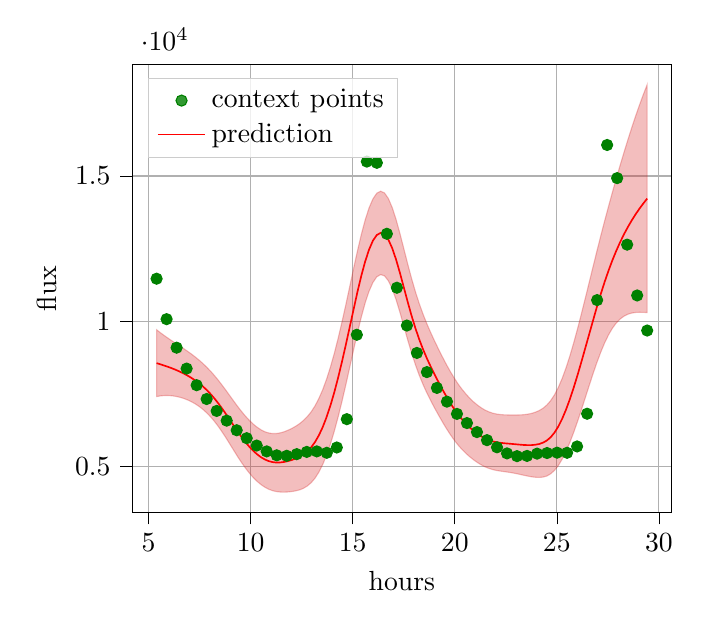
\begin{tikzpicture}

\definecolor{crimson2143940}{RGB}{214,39,40}
\definecolor{darkgray176}{RGB}{176,176,176}
\definecolor{green}{RGB}{0,128,0}
\definecolor{lightgray204}{RGB}{204,204,204}

\begin{axis}[
legend cell align={left},
legend style={
  fill opacity=0.8,
  draw opacity=1,
  text opacity=1,
  at={(0.03,0.97)},
  anchor=north west,
  draw=lightgray204
},
tick align=outside,
tick pos=left,
x grid style={darkgray176},
xlabel={hours},
xmajorgrids,
xmin=4.19309692382812, xmax=30.6273376464844,
xtick style={color=black},
y grid style={darkgray176},
ylabel={flux},
ymajorgrids,
ymin=3400.75622558594, ymax=18855.8233642578,
ytick style={color=black}
]
\addplot [draw=green, fill=green, mark=*, only marks]
table{%
x  y
5.3946533203125 11461
5.885009765625 10066.2001953125
6.3753662109375 9083.2998046875
6.86572265625 8362.2001953125
7.3564453125 7789.7998046875
7.8468017578125 7313.7001953125
8.337158203125 6903
8.8275146484375 6568.10009765625
9.3182373046875 6236.60009765625
9.80859375 5963.39990234375
10.2989501953125 5709.39990234375
10.789306640625 5507.7998046875
11.2796630859375 5372.89990234375
11.7703857421875 5356.39990234375
12.2607421875 5413.60009765625
12.7510986328125 5490.2001953125
13.241455078125 5507.89990234375
13.7318115234375 5459.5
14.2225341796875 5642.10009765625
14.712890625 6619
15.2032470703125 9528.599609375
15.693603515625 15498.7998046875
16.1839599609375 15456.599609375
16.6746826171875 13009.2998046875
17.1650390625 11150.099609375
17.6553955078125 9846.7001953125
18.145751953125 8902.099609375
18.6361083984375 8241.2998046875
19.1268310546875 7696.10009765625
19.6171875 7223.2001953125
20.1075439453125 6800.39990234375
20.597900390625 6484.39990234375
21.0882568359375 6173.2001953125
21.5789794921875 5895.39990234375
22.0693359375 5648.7001953125
22.5596923828125 5439
23.050048828125 5344.2998046875
23.5404052734375 5352.10009765625
24.0311279296875 5430.89990234375
24.521484375 5451.2998046875
25.0118408203125 5463.89990234375
25.502197265625 5459.89990234375
25.9925537109375 5678.2001953125
26.4832763671875 6806.2001953125
26.9736328125 10723.7998046875
27.4639892578125 16070.900390625
27.954345703125 14928.7001953125
28.4447021484375 12635.2001953125
28.9354248046875 10883.2001953125
29.42578125 9674.599609375
};
\addlegendentry{context points}
\path [draw=crimson2143940, fill=crimson2143940, opacity=0.3]
(axis cs:5.3946533203125,9701.65234375)
--(axis cs:5.3946533203125,7397.76513671875)
--(axis cs:5.58387480007382,7421.447265625)
--(axis cs:5.77309627983514,7432.91259765625)
--(axis cs:5.96231775959646,7434.06982421875)
--(axis cs:6.15153923935778,7424.697265625)
--(axis cs:6.34076071911909,7404.48486328125)
--(axis cs:6.52998219888041,7374.28515625)
--(axis cs:6.71920367864173,7334.4619140625)
--(axis cs:6.90842515840305,7283.19287109375)
--(axis cs:7.09764663816437,7221.380859375)
--(axis cs:7.28686811792569,7146.52880859375)
--(axis cs:7.47608959768701,7058.27880859375)
--(axis cs:7.66531107744833,6954.26416015625)
--(axis cs:7.85453255720965,6833.89208984375)
--(axis cs:8.04375403697096,6695.462890625)
--(axis cs:8.23297551673228,6538.1669921875)
--(axis cs:8.4221969964936,6363.0478515625)
--(axis cs:8.61141847625492,6171.18798828125)
--(axis cs:8.80063995601624,5967.28125)
--(axis cs:8.98986143577756,5753.0185546875)
--(axis cs:9.17908291553888,5537.35400390625)
--(axis cs:9.3683043953002,5324.00830078125)
--(axis cs:9.55752587506151,5122.3486328125)
--(axis cs:9.74674735482283,4933.384765625)
--(axis cs:9.93596883458415,4762.01953125)
--(axis cs:10.1251903143455,4609.62890625)
--(axis cs:10.3144117941068,4477.69970703125)
--(axis cs:10.5036332738681,4364.98876953125)
--(axis cs:10.6928547536294,4274.78662109375)
--(axis cs:10.8820762333907,4204.470703125)
--(axis cs:11.0712977131521,4154.67041015625)
--(axis cs:11.2605191929134,4122.4736328125)
--(axis cs:11.4497406726747,4107.4912109375)
--(axis cs:11.638962152436,4103.25927734375)
--(axis cs:11.8281836321973,4110.0673828125)
--(axis cs:12.0174051119587,4123.4765625)
--(axis cs:12.20662659172,4146.599609375)
--(axis cs:12.3958480714813,4180.30078125)
--(axis cs:12.5850695512426,4234.09912109375)
--(axis cs:12.7742910310039,4313.11376953125)
--(axis cs:12.9635125107653,4425.4638671875)
--(axis cs:13.1527339905266,4581.74951171875)
--(axis cs:13.3419554702879,4790.248046875)
--(axis cs:13.5311769500492,5052.8837890625)
--(axis cs:13.7203984298105,5378.77587890625)
--(axis cs:13.9096199095719,5762.09912109375)
--(axis cs:14.0988413893332,6202.55419921875)
--(axis cs:14.2880628690945,6696.9560546875)
--(axis cs:14.4772843488558,7237.49560546875)
--(axis cs:14.6665058286171,7810.26171875)
--(axis cs:14.8557273083784,8407.8271484375)
--(axis cs:15.0449487881398,9010.984375)
--(axis cs:15.2341702679011,9596.630859375)
--(axis cs:15.4233917476624,10142.7294921875)
--(axis cs:15.6126132274237,10627.1396484375)
--(axis cs:15.801834707185,11027.4462890625)
--(axis cs:15.9910561869464,11331.109375)
--(axis cs:16.1802776667077,11525.708984375)
--(axis cs:16.369499146469,11603.783203125)
--(axis cs:16.5587206262303,11557.3291015625)
--(axis cs:16.7479421059916,11389.884765625)
--(axis cs:16.937163585753,11110.234375)
--(axis cs:17.1263850655143,10737.0703125)
--(axis cs:17.3156065452756,10297.9423828125)
--(axis cs:17.5048280250369,9826.466796875)
--(axis cs:17.6940495047982,9352.4287109375)
--(axis cs:17.8832709845595,8904.0947265625)
--(axis cs:18.0724924643209,8494.4345703125)
--(axis cs:18.2617139440822,8129.2890625)
--(axis cs:18.4509354238435,7805.82421875)
--(axis cs:18.6401569036048,7513.3876953125)
--(axis cs:18.8293783833661,7246.60009765625)
--(axis cs:19.0185998631275,6995.1572265625)
--(axis cs:19.2078213428888,6754.5947265625)
--(axis cs:19.3970428226501,6523.0478515625)
--(axis cs:19.5862643024114,6301.6181640625)
--(axis cs:19.7754857821727,6094.673828125)
--(axis cs:19.9647072619341,5905.6904296875)
--(axis cs:20.1539287416954,5733.734375)
--(axis cs:20.3431502214567,5584.19482421875)
--(axis cs:20.532371701218,5449.90185546875)
--(axis cs:20.7215931809793,5329.80419921875)
--(axis cs:20.9108146607406,5222.4638671875)
--(axis cs:21.100036140502,5128.59716796875)
--(axis cs:21.2892576202633,5046.5693359375)
--(axis cs:21.4784791000246,4977.205078125)
--(axis cs:21.6677005797859,4922.52880859375)
--(axis cs:21.8569220595472,4880.662109375)
--(axis cs:22.0461435393086,4850.169921875)
--(axis cs:22.2353650190699,4828.5419921875)
--(axis cs:22.4245864988312,4809.27001953125)
--(axis cs:22.6138079785925,4791.17724609375)
--(axis cs:22.8030294583538,4769.98095703125)
--(axis cs:22.9922509381152,4744.646484375)
--(axis cs:23.1814724178765,4716.5849609375)
--(axis cs:23.3706938976378,4686.6748046875)
--(axis cs:23.5599153773991,4658.576171875)
--(axis cs:23.7491368571604,4633.060546875)
--(axis cs:23.9383583369218,4616.82421875)
--(axis cs:24.1275798166831,4609.62890625)
--(axis cs:24.3168012964444,4620.8515625)
--(axis cs:24.5060227762057,4657.9619140625)
--(axis cs:24.695244255967,4732.24072265625)
--(axis cs:24.8844657357283,4850.55908203125)
--(axis cs:25.0736872154897,5020.4091796875)
--(axis cs:25.262908695251,5240.9833984375)
--(axis cs:25.4521301750123,5510.04638671875)
--(axis cs:25.6413516547736,5822.0908203125)
--(axis cs:25.8305731345349,6173.21142578125)
--(axis cs:26.0197946142963,6552.50537109375)
--(axis cs:26.2090160940576,6954.17919921875)
--(axis cs:26.3982375738189,7367.94677734375)
--(axis cs:26.5874590535802,7783.130859375)
--(axis cs:26.7766805333415,8191.015625)
--(axis cs:26.9659020131029,8577.857421875)
--(axis cs:27.1551234928642,8933.607421875)
--(axis cs:27.3443449726255,9252.392578125)
--(axis cs:27.5335664523868,9525.80078125)
--(axis cs:27.7227879321481,9754.4404296875)
--(axis cs:27.9120094119094,9933.732421875)
--(axis cs:28.1012308916708,10070.8466796875)
--(axis cs:28.2904523714321,10169.990234375)
--(axis cs:28.4796738511934,10236.78515625)
--(axis cs:28.6688953309547,10276.703125)
--(axis cs:28.858116810716,10296.8720703125)
--(axis cs:29.0473382904774,10303.658203125)
--(axis cs:29.2365597702387,10300.859375)
--(axis cs:29.42578125,10292.568359375)
--(axis cs:29.42578125,18153.3203125)
--(axis cs:29.42578125,18153.3203125)
--(axis cs:29.2365597702387,17810.986328125)
--(axis cs:29.0473382904774,17448.361328125)
--(axis cs:28.858116810716,17066.853515625)
--(axis cs:28.6688953309547,16666.45703125)
--(axis cs:28.4796738511934,16249.736328125)
--(axis cs:28.2904523714321,15818.353515625)
--(axis cs:28.1012308916708,15372.9833984375)
--(axis cs:27.9120094119094,14914.681640625)
--(axis cs:27.7227879321481,14444.1123046875)
--(axis cs:27.5335664523868,13957.890625)
--(axis cs:27.3443449726255,13460.9375)
--(axis cs:27.1551234928642,12947.134765625)
--(axis cs:26.9659020131029,12422.041015625)
--(axis cs:26.7766805333415,11884.16015625)
--(axis cs:26.5874590535802,11340.857421875)
--(axis cs:26.3982375738189,10799.1083984375)
--(axis cs:26.2090160940576,10266.1123046875)
--(axis cs:26.0197946142963,9750.443359375)
--(axis cs:25.8305731345349,9261.58984375)
--(axis cs:25.6413516547736,8805.318359375)
--(axis cs:25.4521301750123,8392.7265625)
--(axis cs:25.262908695251,8027.525390625)
--(axis cs:25.0736872154897,7715.189453125)
--(axis cs:24.8844657357283,7457.82763671875)
--(axis cs:24.695244255967,7256.52685546875)
--(axis cs:24.5060227762057,7103.388671875)
--(axis cs:24.3168012964444,6992.861328125)
--(axis cs:24.1275798166831,6912.8671875)
--(axis cs:23.9383583369218,6856.544921875)
--(axis cs:23.7491368571604,6815.3369140625)
--(axis cs:23.5599153773991,6789.6669921875)
--(axis cs:23.3706938976378,6772.8271484375)
--(axis cs:23.1814724178765,6764.6474609375)
--(axis cs:22.9922509381152,6761.1591796875)
--(axis cs:22.8030294583538,6761.06982421875)
--(axis cs:22.6138079785925,6763.14404296875)
--(axis cs:22.4245864988312,6767.72216796875)
--(axis cs:22.2353650190699,6778.408203125)
--(axis cs:22.0461435393086,6796.19921875)
--(axis cs:21.8569220595472,6826.42578125)
--(axis cs:21.6677005797859,6872.03662109375)
--(axis cs:21.4784791000246,6934.001953125)
--(axis cs:21.2892576202633,7014.0419921875)
--(axis cs:21.100036140502,7110.31103515625)
--(axis cs:20.9108146607406,7222.3642578125)
--(axis cs:20.7215931809793,7351.81591796875)
--(axis cs:20.532371701218,7497.86376953125)
--(axis cs:20.3431502214567,7660.98974609375)
--(axis cs:20.1539287416954,7842.080078125)
--(axis cs:19.9647072619341,8047.23828125)
--(axis cs:19.7754857821727,8269.298828125)
--(axis cs:19.5862643024114,8509.5185546875)
--(axis cs:19.3970428226501,8764.0078125)
--(axis cs:19.2078213428888,9028.7998046875)
--(axis cs:19.0185998631275,9303.6103515625)
--(axis cs:18.8293783833661,9591.103515625)
--(axis cs:18.6401569036048,9897.0068359375)
--(axis cs:18.4509354238435,10231.541015625)
--(axis cs:18.2617139440822,10600.314453125)
--(axis cs:18.0724924643209,11013.5263671875)
--(axis cs:17.8832709845595,11473.1201171875)
--(axis cs:17.6940495047982,11972.2041015625)
--(axis cs:17.5048280250369,12496.615234375)
--(axis cs:17.3156065452756,13016.4814453125)
--(axis cs:17.1263850655143,13500.51953125)
--(axis cs:16.937163585753,13913.0390625)
--(axis cs:16.7479421059916,14225.173828125)
--(axis cs:16.5587206262303,14416.9990234375)
--(axis cs:16.369499146469,14478.873046875)
--(axis cs:16.1802776667077,14407.826171875)
--(axis cs:15.9910561869464,14212.15234375)
--(axis cs:15.801834707185,13900.9580078125)
--(axis cs:15.6126132274237,13488.1142578125)
--(axis cs:15.4233917476624,12987.4638671875)
--(axis cs:15.2341702679011,12422.859375)
--(axis cs:15.0449487881398,11817.15625)
--(axis cs:14.8557273083784,11192.7001953125)
--(axis cs:14.6665058286171,10572.640625)
--(axis cs:14.4772843488558,9975.875)
--(axis cs:14.2880628690945,9409.5087890625)
--(axis cs:14.0988413893332,8887.1953125)
--(axis cs:13.9096199095719,8415.876953125)
--(axis cs:13.7203984298105,7998.19677734375)
--(axis cs:13.5311769500492,7634.1767578125)
--(axis cs:13.3419554702879,7329.5791015625)
--(axis cs:13.1527339905266,7075.17529296875)
--(axis cs:12.9635125107653,6869.5751953125)
--(axis cs:12.7742910310039,6705.06591796875)
--(axis cs:12.5850695512426,6571.82177734375)
--(axis cs:12.3958480714813,6463.330078125)
--(axis cs:12.20662659172,6375.21484375)
--(axis cs:12.0174051119587,6299.474609375)
--(axis cs:11.8281836321973,6236.498046875)
--(axis cs:11.638962152436,6183.57958984375)
--(axis cs:11.4497406726747,6146.14453125)
--(axis cs:11.2605191929134,6123.927734375)
--(axis cs:11.0712977131521,6123.02978515625)
--(axis cs:10.8820762333907,6143.5380859375)
--(axis cs:10.6928547536294,6187.49658203125)
--(axis cs:10.5036332738681,6253.49853515625)
--(axis cs:10.3144117941068,6342.94287109375)
--(axis cs:10.1251903143455,6451.1552734375)
--(axis cs:9.93596883458415,6578.654296875)
--(axis cs:9.74674735482283,6723.349609375)
--(axis cs:9.55752587506151,6883.27734375)
--(axis cs:9.3683043953002,7053.91943359375)
--(axis cs:9.17908291553888,7235.39794921875)
--(axis cs:8.98986143577756,7419.6455078125)
--(axis cs:8.80063995601624,7604.8681640625)
--(axis cs:8.61141847625492,7783.77685546875)
--(axis cs:8.4221969964936,7956.205078125)
--(axis cs:8.23297551673228,8118.400390625)
--(axis cs:8.04375403697096,8269.4296875)
--(axis cs:7.85453255720965,8408.67578125)
--(axis cs:7.66531107744833,8536.44140625)
--(axis cs:7.47608959768701,8654.5712890625)
--(axis cs:7.28686811792569,8763.521484375)
--(axis cs:7.09764663816437,8865.412109375)
--(axis cs:6.90842515840305,8960.728515625)
--(axis cs:6.71920367864173,9052.6044921875)
--(axis cs:6.52998219888041,9141.326171875)
--(axis cs:6.34076071911909,9229.1904296875)
--(axis cs:6.15153923935778,9317.650390625)
--(axis cs:5.96231775959646,9407.0439453125)
--(axis cs:5.77309627983514,9500.203125)
--(axis cs:5.58387480007382,9598.375)
--(axis cs:5.3946533203125,9701.65234375)
--cycle;

\addplot [semithick, red]
table {%
5.3946533203125 8549.708984375
5.58387470245361 8509.9111328125
5.77309608459473 8466.5576171875
5.962317943573 8420.556640625
6.15153932571411 8371.173828125
6.34076070785522 8316.837890625
6.52998208999634 8257.8056640625
6.71920347213745 8193.533203125
6.90842533111572 8121.9609375
7.09764671325684 8043.396484375
7.28686809539795 7955.02490234375
7.47608947753906 7856.4248046875
7.66531085968018 7745.3525390625
7.85453271865845 7621.2841796875
8.0437536239624 7482.4462890625
8.23297595977783 7328.28369140625
8.42219734191895 7159.62646484375
8.61141872406006 6977.482421875
8.80064010620117 6786.07470703125
9.36830425262451 6188.9638671875
9.55752563476562 6002.81298828125
9.74674701690674 5828.3671875
9.93596839904785 5670.3369140625
10.1251907348633 5530.39208984375
10.3144121170044 5410.3212890625
10.5036334991455 5309.24365234375
10.6928548812866 5231.1416015625
10.8820762634277 5174.00439453125
11.0712976455688 5138.85009765625
11.26051902771 5123.20068359375
11.4497404098511 5126.81787109375
11.6389617919922 5143.41943359375
11.8281831741333 5173.28271484375
12.0174055099487 5211.4755859375
12.2066268920898 5260.9072265625
12.395848274231 5321.8154296875
12.5850696563721 5402.96044921875
12.7742910385132 5509.08984375
12.9635124206543 5647.51953125
13.1527338027954 5828.46240234375
13.3419551849365 6059.91357421875
13.5311765670776 6343.5302734375
13.7203989028931 6688.486328125
13.9096202850342 7088.98779296875
14.0988416671753 7544.875
14.2880630493164 8053.232421875
14.4772844314575 8606.685546875
14.6665058135986 9191.451171875
15.234169960022 11009.7451171875
15.4233913421631 11565.0966796875
15.6126136779785 12057.626953125
15.8018350601196 12464.2021484375
15.9910564422607 12771.630859375
16.1802768707275 12966.767578125
16.369499206543 13041.328125
16.5587215423584 12987.1640625
16.7479419708252 12807.529296875
16.9371643066406 12511.63671875
17.1263847351074 12118.794921875
17.3156070709229 11657.2119140625
17.6940498352051 10662.31640625
17.8832702636719 10188.607421875
18.0724925994873 9753.98046875
18.2617130279541 9364.8017578125
18.4509353637695 9018.6826171875
18.640157699585 8705.197265625
18.8293781280518 8418.8515625
19.0186004638672 8149.3837890625
19.207820892334 7891.697265625
19.3970432281494 7643.52783203125
19.5862636566162 7405.568359375
19.7754859924316 7181.986328125
19.9647064208984 6976.46435546875
20.1539287567139 6787.9072265625
20.3431510925293 6622.59228515625
20.5323715209961 6473.8828125
20.7215938568115 6340.81005859375
20.9108142852783 6222.4140625
21.1000366210938 6119.4541015625
21.2892570495605 6030.3056640625
21.478479385376 5955.603515625
21.6676998138428 5897.28271484375
21.8569221496582 5853.5439453125
22.0461444854736 5823.1845703125
22.2353649139404 5803.47509765625
22.4245872497559 5788.49609375
22.8030300140381 5765.525390625
23.1814727783203 5740.6162109375
23.3706932067871 5729.7509765625
23.5599155426025 5724.12158203125
23.7491359710693 5724.19873046875
23.9383583068848 5736.6845703125
24.1275806427002 5761.248046875
24.316801071167 5806.8564453125
24.5060234069824 5880.67529296875
24.6952438354492 5994.3837890625
24.8844661712646 6154.193359375
25.0736865997314 6367.79931640625
25.2629089355469 6634.25439453125
25.4521293640137 6951.38671875
25.6413516998291 7313.70458984375
25.8305740356445 7717.40087890625
26.0197944641113 8151.474609375
26.2090167999268 8610.1455078125
26.9659023284912 10499.94921875
27.155122756958 10940.37109375
27.3443450927734 11356.6650390625
27.5335655212402 11741.845703125
27.7227878570557 12099.2763671875
27.9120101928711 12424.20703125
28.1012306213379 12721.9150390625
28.2904529571533 12994.171875
28.4796733856201 13243.2607421875
28.6688957214355 13471.580078125
28.8581161499023 13681.86328125
29.0473384857178 13876.009765625
29.2365589141846 14055.9228515625
29.42578125 14222.9443359375
};
\addlegendentry{prediction}
\end{axis}

\end{tikzpicture}

	}
	\caption{Model A Prediction result on luminosity values (unit flux) for a cepheid variable star over 24 hours. Data from Benkő et al. \cite{Benk__2014}}
	\label{fig:cepheid}
\end{figure}

To apply our model to real-world data and seriously test its generalization capabilities, we process Cepheid star luminosity data. \autoref{fig:cepheid} shows prediction results for Model-A. Due to missing ground truth data, we cannot evaluate the performance numerically. We observe a comparatively high uncertainty despite a high number of context points, especially during the low luminosity phases. Otherwise, these results show good generalization from training on synthetic data and applying the same model on real world observations.

